\documentclass[11pt]{article}

\usepackage{comment} % enables the use of multi-line comments (\ifx \fi) 
\usepackage[a4paper,margin=1cm]{geometry}
\usepackage[utf8]{inputenc}
\usepackage[ngerman]{isodate}
\usepackage{gensymb}
\usepackage{graphicx}
\usepackage{booktabs}% http://ctan.org/pkg/booktabs
\usepackage{tabularx}
\usepackage{ltablex} % Longtables with tabularx
\usepackage[x11names]{xcolor}
\usepackage{amsmath}
\usepackage{amssymb}
\usepackage{amsthm}
\usepackage{array}
\usepackage{wrapfig}
\usepackage{subcaption}
\usepackage{csquotes}
\usepackage{pdflscape}
\usepackage{geometry}
\usepackage{multicol}
\usepackage{bm}
\usepackage{enumitem}
\usepackage{hyperref}
\usepackage{mdframed}
\usepackage{scalerel}
\usepackage{stackengine}
\usepackage{mathtools}
\usepackage{pdfpages}
\usepackage{xcolor}

% Code highlighting
\usepackage{minted}

% Be able to caption equations and float them in place
\usepackage{float}

\newmdtheoremenv{theorem}{Theorem}

% improved "definition" element with colored, thicker border
%\theoremstyle{definition}
%\newmdtheoremenv[%
%backgroundcolor=white,
%linecolor=teal,
%linewidth=2pt]{definition}{}%[section]

% simple frame around definition

\newmdenv[%
linecolor=teal!50,
backgroundcolor=teal!20,
linewidth=1.5pt]{definition}

% Define the frame style for R code snippets
\mdfdefinestyle{mystyle}{
	linewidth=1.5pt,
	linecolor=red,
	% Other style options can be added here
}

% Define a new environment for R code snippets with mdframed
\AtBeginEnvironment{minted}{\let\itshape\relax} % disable italics in minted elements
\mdfdefinestyle{code-frame}{
	linewidth=1.5pt,
	linecolor=orange,
	% Other style options can be added here
}
\surroundwithmdframed[style=code-frame]{minted}


\geometry{a4paper, margin=2.0cm}

\newcommand\equalhat{\mathrel{\stackon[1.5pt]{=}{\stretchto{\scalerel*[\widthof{=}]{\wedge}{\rule{1ex}{3ex}}}{0.5ex}}}}
\newcommand\defeq{\mathrel{\overset{\makebox[0pt]{\mbox{\normalfont\tiny def}}}{=}}}
\newcolumntype{C}{>{\centering\arraybackslash}X}

\newcommand*\samplemean[1]{\overline{#1}}
\newcommand*\ev[1]{\mathrel{\text{E}\left[#1\right]}}
\newcommand*\R{\mathbb{R}}
\newcommand*\Z{\mathbb{Z}}
\newcommand*\N[1]{\mathcal{N}\left(#1\right)}
\newcommand*\F[1]{\mathcal{F}_{#1}}
\newcommand*\Likelihood{\mathcal{L}}
\newcommand*\diff{\mathop{}\!\mathrm{d}}
\newcommand*\Diff[1]{\mathop{}\!\mathrm{d^#1}}
\newcommand*\Exp[1]{\mathop{\text{Exp}}\left(#1\right)}
\newcommand*\Cov[1]{\mathop{\text{Cov}}\left(#1\right)}
\newcommand*\Cor[1]{\mathop{\text{Cor}}\left(#1\right)}
\newcommand*\Var[1]{\mathop{\text{Var}}\left(#1\right)}
\newcommand*\Std[1]{\mathop{\text{Std}}\left(#1\right)}
\newcommand*\predvar[1]{{\color{SeaGreen4} \texttt{#1}}}
\newcommand{\overbar}[1]{\mkern 1.5mu\overline{\mkern-1.5mu#1\mkern-1.5mu}\mkern 1.5mu}

\DeclarePairedDelimiter\abs{\lvert}{\rvert}
\DeclarePairedDelimiter\norm{\lVert}{\rVert}

\setcounter{tocdepth}{3}
\setcounter{secnumdepth}{3}

\graphicspath{{./img/}}

\begin{document}
	
\title{Predictive Modeling FS24}
\author{Pascal Baumann\\pascal.baumann@stud.hslu.ch\\\\Thomas Annen\\thomas.annen@stud.hslu.ch}
\maketitle



For errors or improvement raise an issue or make a pull request on the \href{https://github.com/KilnOfTheSecondFlame/mse_summaries}{github repository}.

\tableofcontents
\newpage



%\section{Introduction}
%Statistical Modeling means finding a density function that produces your given data. From Wikipedia:

% "Predictive modeling uses statistics to predict outcomes. Most often the event one wants to predict is in the future, but predictive modelling can be applied to any type of unknown event, regardless of when it occurred. In many cases the model is chosen on the basis of detection theory to try to guess the probability of an outcome given a set amount of input data."

%Predictive modeling is done with Supervised Models, the major challenge in using data to make predictions is distinguishing what is a meaningful signal from the noise.

\section{Probability Models for Measurement Data}

\subsection{Continuous Random Variables and Probability Distributions}

\begin{definition}
	\textbf{Bracket notation:}\\
	An interval $(a, b]$ contains all points $x$ with $x > a$ and $x \leq b$.
\end{definition}

\subsubsection{Probability Density}

\begin{definition}
	\textbf{Probability Density Function}\\
	The probability density $f$ is defined as the derivative of the cumulative distribution function:
	\begin{equation*}
		f(x) = F'(x)
	\end{equation*}
\end{definition}

$F(x)$ describes the cumulative distribution function (CDF). Exemplary CDF:

\begin{center}
	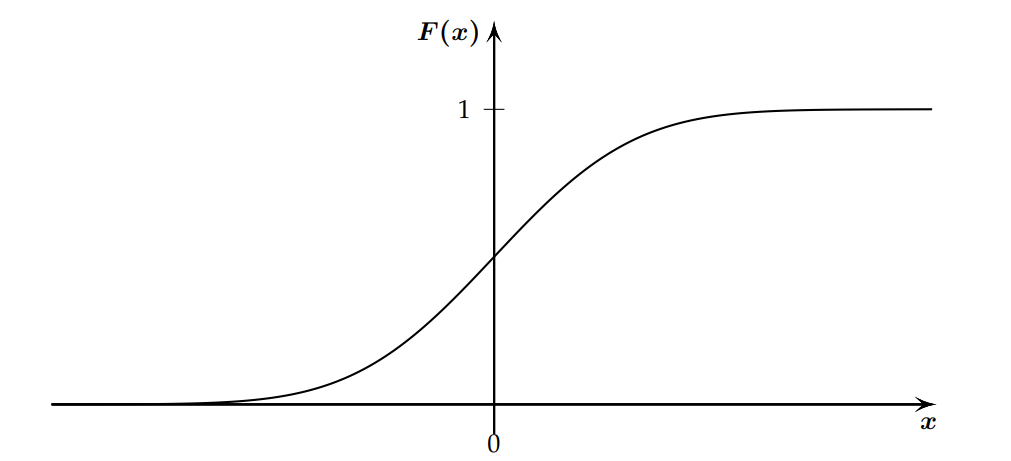
\includegraphics[width=0.5\linewidth]{img/cdf}
\end{center}

\begin{definition}
	\textbf{Properties of Probability Density Function}
	\begin{enumerate}
		\item $f(x) \geq 0\quad \text{for all }x$
		\item $P(a<X\leq b) = F(b) - F(a) = \int_{a}^{b}f(x) dx\quad;\quad \text{area between }a\ \text{and }b\ \text{under }f(x)$
		\item $ \int_{-\infty}^{\infty}f(x) dx = 1$
	\end{enumerate}
\end{definition}


\subsubsection{Summary Statistics of Continuous Distributions}

\begin{definition}
	\textbf{Expected value and variance}
	\begin{equation*}
		\ev{X} = \int_{-\infty}^{\infty} x\cdot f(x) dx
	\end{equation*}
	\begin{equation*}
		\text{Var}(X) = \sigma_X^2 = \ev{((X - \ev{X})^2} = \int_{-\infty}^{\infty} (x - \ev{X})^2 f(x) dx = \ev{X^2} - \ev{X}^2
	\end{equation*}
	A \textbf{quantile} $q(\alpha) (0<\alpha<1)$ of a continuous random variable $X$, respectively of a probability distribution is defined as
	\begin{equation*}
		P(X\leq q(\alpha)) = \alpha \Leftrightarrow F(q(\alpha)) = \alpha \Leftrightarrow q(\alpha) = F^{-1}(\alpha)
	\end{equation*}
\end{definition}


Interpretation of quantiles:
\begin{center}
	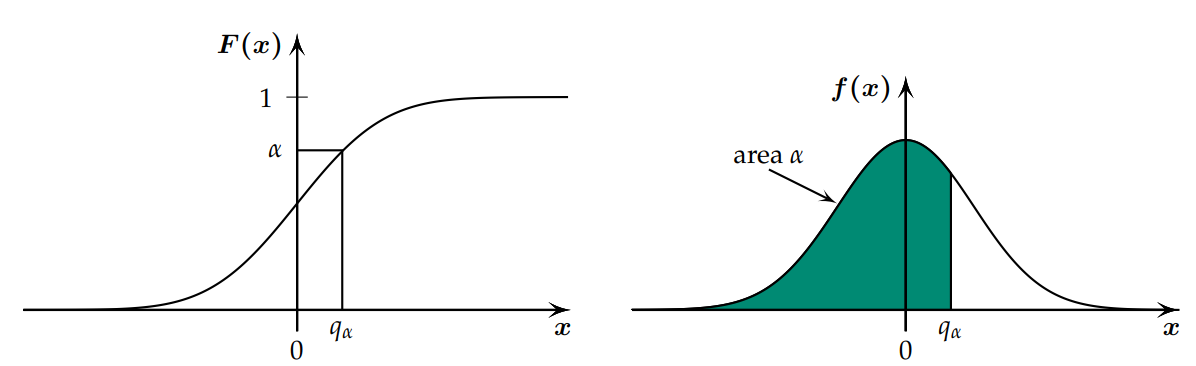
\includegraphics[width=0.8\linewidth]{img/quantile}
\end{center}

\subsection{Important Continuous Distributions}


% The set of all possible outcomes of a random experiment is called sample space $\omega$. Random variables $X$ are real-valued functions on $\omega$. $W_X$ is the value range, that is the set of all values which $X$ can take on. If $W_X$ is discrete then $X$ is called a \emph{discrete} random variable. A probability mass function (PMF) is the probability that $X$ takes on a given value and is written as $P(X=k)$, a probability distribution is the cumulative PMF for all values $x$ in $W_X$.

%\begin{definition}
%	The \textbf{sample total} is defined as 
%	\begin{equation*}
%		S_n = (X_1 + X_2 + \dots + X_n) \sim \N{n\mu, n\sigma_X^2}
%	\end{equation*}
%	\textbf{Sample mean} is defined by
%	\begin{equation*}
%		\samplemean{X}_n = \frac{S_n}{n} \sim(\mu, \frac{\sigma_X^2}{n})
%	\end{equation*}
%	\textbf{Law of Large Numbers} states that
%	\begin{equation*}
%		\samplemean{X}_n \longrightarrow \mu(n\rightarrow \infty)
%	\end{equation*}
%\end{definition}

\subsubsection{Uniform Distribution}
The uniform distribution represents a probabilistic formulation of complete lack of bias or knowledge
\begin{definition}
	A random variable $X$ with range $W_X = [a,b]$ is uniformly distributed if
	\begin{equation*}
		f(x) = \left\{
			\begin{matrix}
				\frac{1}{b-a} & \text{if } a\leq x \leq b\\
				0 & \text{otherwise}
			\end{matrix}
		\right.
	\end{equation*}
\end{definition}
The density function is therefore constant on the interval $[a,b]$, hence the name \emph{uniform}. The corresponding cumulative distribution function is given by
\begin{equation*}
	F(x) = \left\{
		\begin{matrix}
			0 & \text{if } x < a\\
			\frac{x-a}{b-a} & \text{if } a\leq x \leq b\\
			1 & \text{if } x > b
		\end{matrix}
		\right.
\end{equation*}

For $X \thicksim \text{Uniform}([a, b])$, the summary statistics are given by:
\begin{gather*}
	\ev{X} = \frac{a+b}{2}\\
	\Var{X} = \frac{(b-a)^2}{12}\\
	\sigma_X = \frac{b-a}{\sqrt{12}}
\end{gather*}

With R the \textit{value} of the \textit{probability density function} Uniform$([1, 10])$ at the position $x$ = 5 can be calculated as follows:
\begin{minted}{R}
dunif(x=5, min=1, max=10)
## [1] 0.111
\end{minted}

Example with $X \thicksim$ Uniform$([1, 10])$, the probability $P(1.2 \leq X \leq 4.8)$ is:
\begin{minted}{R}
punif(q=4.8, min=1, max=10) - punif(q=1.2, min=1, max=10)
## [1] 0.4
\end{minted}

Generate uniformly distributed random variables: 
\begin{minted}{R}
runif(5,min=1,max=10)
## [1] 9.022951 1.567384 4.828237 2.784172 6.743325
\end{minted}



\subsubsection{Exponential Distribution}
The exponential distribution is used to model the lifespan or time until failure.
\begin{definition}
	A random variable $X$ with range $W_X = \R^+ = [0,\infty)$ is exponentially distributed with parameter $\lambda \in \R^+$ if
	\begin{equation*}
		f(x) = \left\{
			\begin{matrix}
			\lambda\cdot e^{-\lambda x} & \text{if } x\geq 0\\
			0 & \text{otherwise}
			\end{matrix}
		\right.
	\end{equation*}
	We write: 
	\begin{equation*}
		X \thicksim \text{Exp}(\lambda)
	\end{equation*}
		
\end{definition}
The corresponding cumulative distribution function is given by
\begin{equation*}
		F(x) = \left\{
		\begin{matrix}
			1 - e^{-\lambda x} & \text{if } x\geq 0\\
			0 & \text{if } x < 0
		\end{matrix}
	\right.
\end{equation*}
For $X \thicksim \text{Exp}(\lambda)$ the summary statistics are shown below:
\begin{gather*}
	\ev{X} = \frac{1}{\lambda}\\
	\Var{X} = \frac{1}{\lambda^2}\\
	\sigma_X = \frac{1}{\lambda}
\end{gather*}

(Left): Density distribution function of the exponential distribution for $\lambda$ = 1 (green),
$\lambda$ = 2 (blue dashed) and $\lambda$ = 1/2 (violet dotted). (Right): Cumulative distribution
function for the exponential distribution.
\begin{center}
	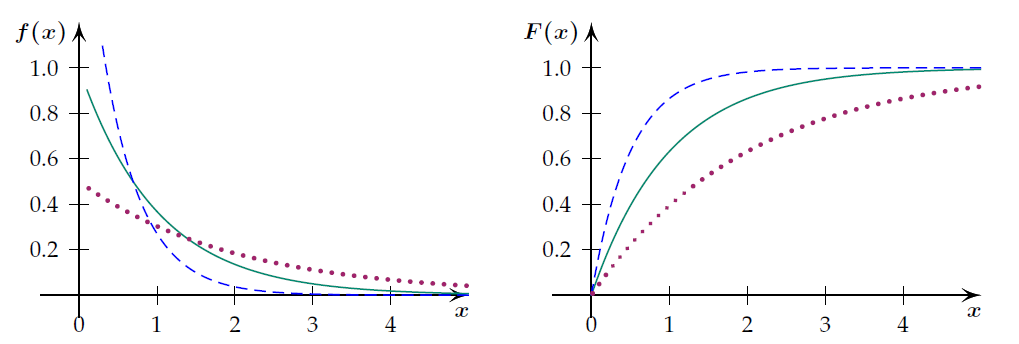
\includegraphics[width=0.9\linewidth]{img/exp-distribution}
\end{center}

Assuming  $X \thicksim \text{Exp}(3)$, the probability $P(0 \leq X \leq 4)$ can be calculated in R as follows:
\begin{minted}{R}
pexp(4, rate=3)
## [1] 0.9999939
\end{minted}



\subsubsection{Normal Distribution (Gaussian)}
The normal distribution or Gaussian distribution is the most frequent distribution occurring with measurement values.
\begin{definition}
	A random variable $X$ with range $W_X = \R$ is normally distributed with parameter $\mu \in \R$ and $\sigma^2\in\R^+$ if
	\begin{equation*}
	f(x) = \frac{1}{\sqrt{2\pi} \sigma} e^{\left( -\frac{(x-\mu)^2}{2\sigma^2} \right)}
	\end{equation*}
	Notation \& cumulative distribution function:
	\begin{equation*}
		X \sim \N{\mu,\sigma^2} \quad \quad \quad \quad F(x) = \int_{-\infty}^{x} f(y)\cdot dy
	\end{equation*}
\end{definition}

For $X \sim \N{\mu,\sigma^2}$ the summary statistics are shown below:
\begin{gather*}
	\ev{X} = \mu\\
	\Var{X} = \sigma^2\\
	\Std{X}=\sigma_X = \sigma
\end{gather*}

Additionally, the following rules hold:
\begin{gather*}
	P(\mu-\sigma \leq X \leq \mu+\sigma) \approx 0.66\\
	P(\mu-2 \sigma \leq X \leq \mu+2 \sigma) \approx 0.95
\end{gather*}

Densities (left) and cumulative distribution functions (right) of the normal distributions for $\mu = 0$, $\sigma = 1$ (green), $\mu = 0$, $\sigma = 2$ (blue), $\mu = 0$, $\sigma = 0.75$ (violet) and $\mu = 33$, $\sigma = 1$  (red):

\begin{center}
	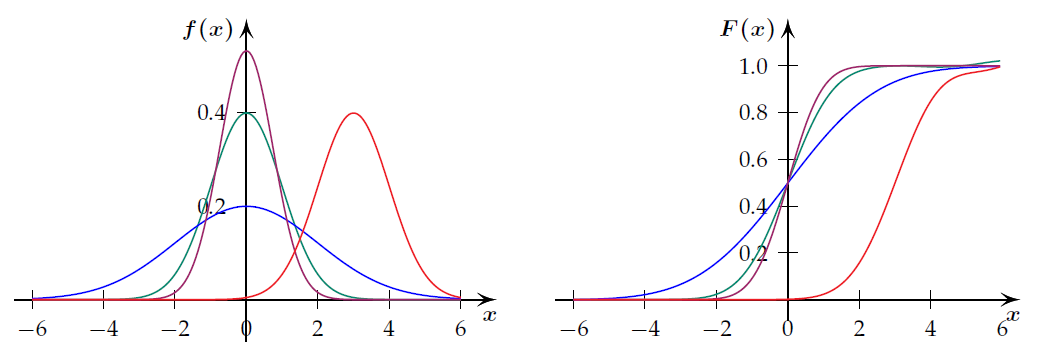
\includegraphics[width=0.9\linewidth]{img/gaussian-distribution}
\end{center}

Assuming $X \sim \N{100, 15^2}$ for the IQ of people, we want to find $P(X > 130)$.
As $P(X > 130) = 1 - P(X < 130)$, we calculate it in R:
\begin{minted}{R}
1 - pnorm(130, mean=100, sd=15)
## [1] 0.02275013
\end{minted}

\subsection{Linear Transformations of single random variable}

\subsubsection{Transformations on Summary Statistics}
\begin{definition}
	\textbf{Properties of Linear Transformations of a Random Variable:}\\
	For $Y=a+b X$, the following relations apply:
	\begin{enumerate}[label=(\roman*)]
		\item $\mathrm{E}(Y)=\mathrm{E}(a+b X)=a+b \mathrm{E}(X)$
		\item $\operatorname{Var}(Y)=\operatorname{Var}(a+b X)=b^2 \operatorname{Var}(X), \quad \sigma_Y=|b| \sigma_X$
		\item $\alpha - \text{Quantile of } Y=q_Y(\alpha)=a+b q_X(\alpha)$
		\item $f_Y(y)=\frac{1}{b} f_X\left(\frac{y-a}{b}\right)$
	\end{enumerate}
\end{definition}

\subsubsection{Standardization of A Normally Distributed Random Variable}
\begin{definition}
	Standardizing $ X\sim\N{\mu,\sigma^2} $ results in a transformed random variable that is normally distributed with expected value zero and the variance one:
	\begin{equation*}
		Z = \frac{X - \mu}{\sigma} \sim \N{0,1}
	\end{equation*}
\end{definition}

\textbf{Example:} If $X \sim \mathcal{N}\left(\mu, \sigma^2\right)$ with $\mu=2$ and $\sigma^2=4$, then:
\begin{equation*}
	P(X \leq 5)=P\left(\frac{X-\mu}{\sigma} \leq \frac{5-\mu}{\sigma}\right)=P\left(Z \leq \frac{5-2}{2}\right)=P(Z \leq 1.5)=\Phi(1.5)=0.93
\end{equation*}
$\Phi$ is the CDF, calculation in R: 
\begin{minted}{R}
pnorm(1.5, 0, 1)
## [1] 0.9331928
\end{minted}

\subsection{Non-Linear Transformations}

\begin{definition}
	\textbf{General Transformations of a Random Variable:}\\
	Let us consider the general transformation of a random variable $X$:
	\begin{equation*}
		Y=g(X)
	\end{equation*}
	
	The cumulative distribution function and the density of $Y$ are determined by the density distribution function of $X$. The following formula can always be used for the calculation of the expected value
	\begin{equation*}
		\mathrm{E}(Y)=\mathrm{E}(g(X))=\int_{-\infty}^{\infty} g(x) f_X(x) \mathrm{d} x
	\end{equation*}
\end{definition}

\subsection{Functions of Several Random Variables}
\subsubsection{Independence and i.i.d. Assumption}
If the random variables $X_1, \ldots, X_n$ are independent and all follow the same distribution, we use the following notation $X_1, \ldots, X_n \text{ i.i.d. }$. The abbreviation \textbf{i.i.d.} stands for:
\begin{center}
\textbf{i}ndependent, \textbf{i}dentically \textbf{d}istributed
\end{center}

\noindent
The following relation is always true:
$$
\mathrm{E}\left(X_1+X_2\right)=\mathrm{E}\left(X_1\right)+\mathrm{E}\left(X_2\right)
$$
The following relation only holds, if $X_1$ and $X_2$ are independent:
$$
\operatorname{Var}\left(X_1+X_2\right)=\operatorname{Var}\left(X_1\right)+\operatorname{Var}\left(X_2\right)
$$

\subsubsection{Summary Statistics of $S_n$ and $\bar{X}_n$}

\begin{definition}
	\textbf{Summary Statistics of the Sample Total $S_n$:}\\
	For random variables $X_1,X_2,\dots,X_n$ i.i.d.:
	\begin{align*}
		\ev{S_n} &= \ev{X_1 + X_2 + \dots + X_n} = \sum_{i=1}^{n} \ev{X_i} = n\mu\\
		\Var{S_n} &= \sum_{i=1}^{n}\Var{X_i} = n\Var{X_i} = n\sigma_X^2\\
		\sigma(S_n) &= \sqrt{n}\sigma_X
	\end{align*}
\end{definition}

\begin{definition}
	\textbf{Summary Statistics of the Sample Mean $\samplemean{X}_n$}\\
	The standard deviation of $\samplemean{X}_n$ is called the standard error of the sample mean.
	\begin{align*}
		\ev{\samplemean{X}_n} &= \ev{\frac{X_1 + X_2 + \dots + X_n}{n}} = \frac{1}{n} \sum_{i=1}^{n} \ev{X_i} = \mu\\
		\Var{\samplemean{X}_n} &= \Var{\frac{X_1 + X_2 + \dots + X_n}{n}} = \frac{1}{n^2} \sum_{i=1}^{n}\Var{X_i} = \frac{1}{n^2}n\sigma_X^2 = \frac{\sigma_X^2}{n}\\
		\sigma (\samplemean{X}_n) &= \frac{\sigma_X}{\sqrt{n}} = \frac{1}{\sqrt{n}} \sigma_X
	\end{align*}
\end{definition}

\begin{definition}
	\textbf{Law of Large Numbers}\\
	For $n\rightarrow\infty$ the dispersion of the random variables approaches zero. If $X_1,X_2,\dots,X_n$ are i.i.d. then the \textbf{law of large numbers} applies:
	\begin{equation*}
		\samplemean{X}_n \longrightarrow \mu \qquad\text{for} (n\rightarrow\infty)
	\end{equation*}
\end{definition}

\begin{definition}
	\textbf{Standard Error}\\
	The standard deviation of the sample mean (\textit{standard error}) is, however, \textit{not} proportional
	to $1/n$ but decreases only by the factor $1/\sqrt{n}$. To halve the standard error, one needs four times as many observations. This is also known as the $\sqrt{n}$-law.
	\begin{equation*}
		\sigma (\samplemean{X}_n) = \sigma_{\samplemean{X}_n} = \frac{\sigma_X}{\sqrt{n}} = \frac{1}{\sqrt{n}} \sigma_X
	\end{equation*}
\end{definition}

\subsubsection{Central Limit Theorem}
\begin{definition}
	Let $X_1,X_2,\dots,X_n$ be i.i.d. with expected value $\mu$ and variance $\sigma^2$, then
	\begin{align*}
		S_n &\approx \N{n \cdot \mu, n \cdot \sigma_X^2}\\
		\samplemean{X}_n &\approx \N{\mu,\frac{\sigma_X^2}{n}}
	\end{align*}
	This approximation becomes more precise the larger $n$ is. Moreover, the approximation is better, the more the distribution of the random variable $X_i$ is similar to a normal distribution $\N{\mu,\sigma_X^2}$.
\end{definition}


\noindent
\textbf{Example:} What is the probability that among 10000 tosses of a fair coin, heads would appear in maximum 5100 cases? The number of tosses of a coin in which heads appear follows a $\operatorname{Bin}(10000,0.5)$ distribution. We approximate this distribution as a normal distribution, i.e.,
$$
X \sim \mathcal{N}\left(\mu, \sigma^2\right)
$$
with
$$
\mu=10000 \cdot 0.5=5000 \text { and } \sigma^2=10000 \cdot 0.5 \cdot(1-0.5)=2500
$$

\noindent
And we obtain
$$
X \sim \operatorname{Bin}(10000,0.5) \approx \mathcal{N}(5000,2500)
$$

\noindent
We are interested in the probability
$$
P(X \leq 5100)=\Phi\left(\frac{5100-5000}{\sqrt{2500}}\right)=\Phi(2) \approx 0.98
$$


\begin{minted}{R}
pnorm(5100,5000,sqrt(2500)) # approximated calculation
## [1] 0.9772499

pbinom(5100,10000,.5) # exact calculation
## [1] 0.9777871
\end{minted}

\subsection{Distribution Summary}

\begin{center}
	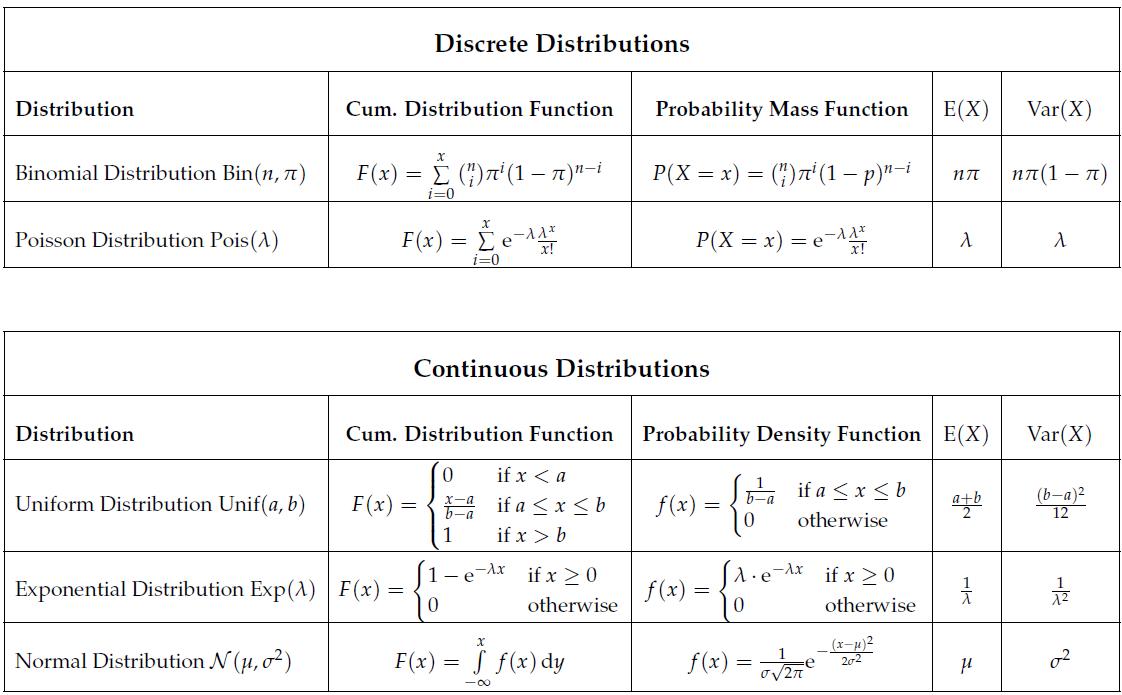
\includegraphics[width=1.0\linewidth]{img/distribution-summary}
\end{center}

\newpage
\section{Statistics for Measurement Data}

\subsection{Assess the Normal Distribution Assumption}
% \section{QQ-Plots, Parameter Estimation and t-Tests}
\subsubsection{QQ-Plot}

A QQ-plot is the empirical quantiles calculated from the data, plotted against the theoretical quantiles. If the data is normal distributed the resulting plot has a linear relationship.

\begin{enumerate}[label=(\arabic*)]
	\item Data set $x_1,x_2,\dots, x_n$ ordered from small to large.
	\item $\alpha_k = \frac{k-0.5}{n}\quad \text{with } k=1,2,\dots,n$
	\item Theoretical Quantile $q(\alpha_k) = \Phi^{-1}(\alpha_k)$
	\item Empirical Quantile $x_{(1)}, x_{(2)},\dots, x_{(n)}$
	\item Plot $\left( q(\alpha_k), x_{(k)} \right)$ to get the QQ-Plot.
\end{enumerate}

\begin{minted}{R}
# Values orded by size:
x <- c(24.4, 27.6, 27.8, 27.9, 28.5, 30.1, 30.3, 31.7, 32.2, 32.8, 33.3, 
  33.5, 34.1, 34.6, 35.8, 35.9, 36.8, 37.1, 39.2, 39.7)

# Quantiles
alpha_k <- (seq(1, length(x),by=1)-0.5)/length(x)
quantile_theor <- qnorm(alpha_k, mean=mean(x),sd=sd(x))
quantile_empir <- sort(x)

# Q-Q-Plot
qqplot(quantile_theor, quantile_empir, xlab="Theoritcal Quantile",
  ylab="Empirical Quantile")
\end{minted}

\subsubsection{Normal Plot}
Special case of QQ-plot, where the empirical quantiles are plotted against the quantiles of the standard normal distribution $X \sim \mathcal{N}\left(0, 1\right)$. If we generate a normal plot, the points in the normal plot will lie approximately on a straight line having axis intercept $\mu$ and slope $\sigma$, when we have a normal distribution.


\textit{Left:} Normal plot for 50 realizations of N(0, 1). The dots lie on a straight line.

\textit{Right:} A distribution which is very long-tailed, dots do not form a straight line.
\begin{center}
	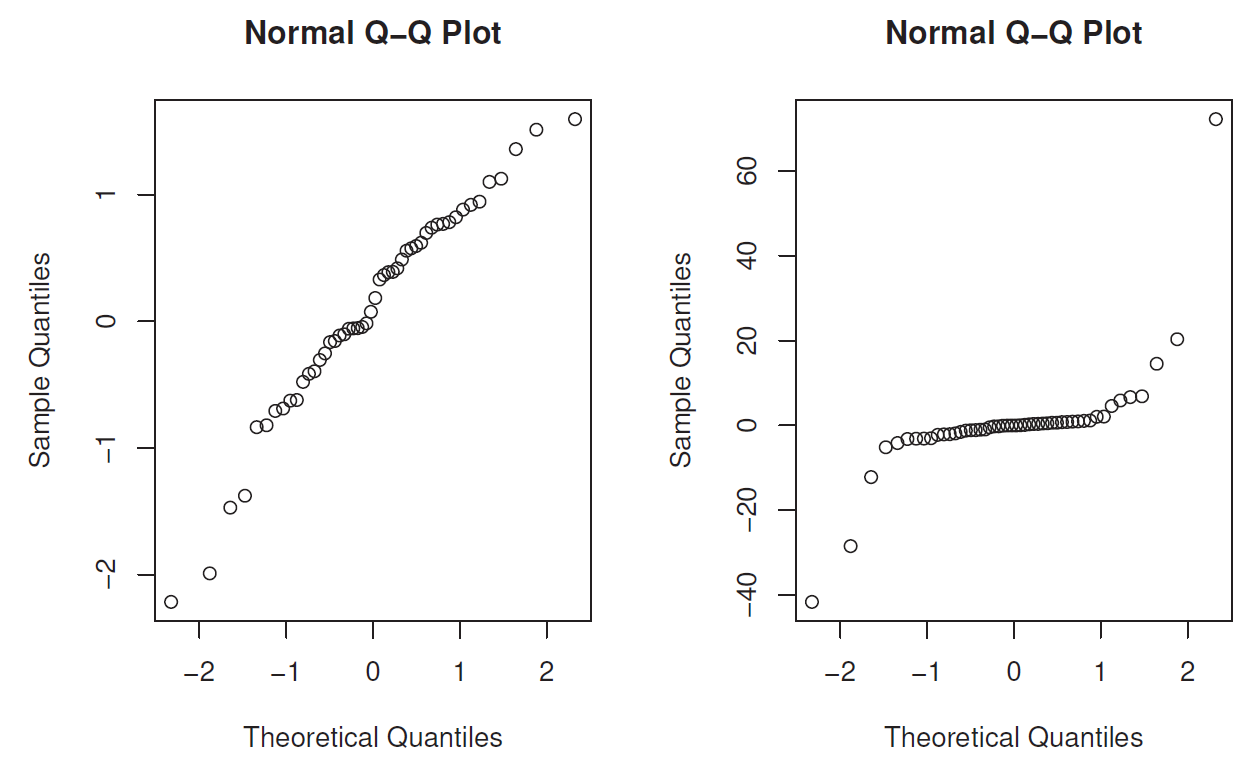
\includegraphics[width=0.7\linewidth]{img/qq-plot-comparison}
\end{center}

\subsection{Parameter Estimation}

\subsubsection{Method of Moments}
We simply use the following formulas to estimate the parameters: 
\begin{equation*}
	\mu = \ev{X} \Rightarrow \hat{\mu} = \bar{x}_n = \dfrac{x_1+x_2 + ... + x_n}{n}\\
\end{equation*}
\begin{align*}
	\sigma_X^2 &= \ev{X^2} - \ev{X}^2\\
	 &= \ev{X^2} - \mu^2
\end{align*}

\noindent
For an \textbf{exponential distribution}, we simply use:
\begin{equation*}
	\ev{X} = \dfrac{1}{\lambda} \Rightarrow \hat{\lambda} = \dfrac{1}{\hat{x}}
\end{equation*}

\subsubsection{Method of Maximum Likelihood}
For a discrete probability distribution, the probability that these $n$ observations or events actually have occurred can be expressed as:
\begin{equation*}
	P[X_1 = x_1] \cdot P[X_2 = x_2] \cdot ... \cdot P[X_n = x_n] \equiv \prod_{i=1}^{n} P[X_i = x_i]
\end{equation*}

The probability that $x_1,x_2,\dots,x_n$ are observed depends on the \textbf{parameter $\theta$} which needs to be \textbf{estimated}. The Likelihood function $\Likelihood(\theta)$ which we want to maximize is given by:
\begin{equation*}
	\Likelihood(\theta) = \prod_{i=1}^{n} P[X_i = x_i | \theta ]
\end{equation*}

\begin{definition}
	\textbf{For Continuous Distribution}\\
	Given a continuous probability distribution  with probability density function $f (x;\theta)$, then the probability that each observation $x_i$ falls into its corresponding interval $[x_i, x_i + \text{d}x_i]$ is
	\begin{equation*}
		\prod_{i=1}^{n} f(x_i; \theta) \text{d}x_i \quad \quad \text{or, as d} x_i \text{ is small and does not contain }\theta \text{: } \Likelihood(\theta) = \prod_{i=1}^{n} f(x_i;\theta)
	\end{equation*}
\end{definition}

\begin{definition}
	\textbf{For Exponential Distribution}\\
	Given observation $X_1, X_2, \dots, X_n\ \text{i.i.d.}\ \sim \Exp{\lambda}$, that is $f(x_i;\lambda) = \lambda e^{-\lambda x_i}$. The \textbf{likelihood function} for such a dataset is given by
	\begin{equation*}
		\Likelihood(\lambda) = \prod_{i=1}^{n} \lambda e^{-\lambda x_i}
	\end{equation*}
	
	\noindent
	The \textbf{Log likelihood} is
	\begin{equation*}
		\log(\Likelihood(\lambda)) = n\log(\lambda) - \lambda\sum_{i=1}^n x_i
	\end{equation*}
	
	\noindent
	The maximum likelihood estimate $\hat{\lambda}$ corresponds to the result with "Method of Moments".
\end{definition}

\subsection{Statistical Tests and Confidence Interval for normally distributed data}
Whenever we record a new measurement series for the same experiment, we will obtain different values (realizations) of $\hat{\mu}$ and $\hat{\sigma}^2_X$. We want to specify a \textit{confidence interval} for the estimate $\hat{\mu}$ that contains the true value of $\mu$ with a certain probability. We can also check if a realization of $\mu$ is compatible with the assumed value $\mu_0$ using a \textit{statistical test}.
\begin{equation*}
	\hat{\mu} = \frac{1}{n} \sum_{i=1}^{n}X_i \qquad \qquad
	\hat{\sigma}^2_X = \frac{1}{n-1} \sum_{i=1}^{n}\left(X_i-\overbar{X}_n\right)^2
\end{equation*}


\subsubsection{z-Test ($\sigma_X$ known)}

\begin{enumerate}[label=\textbf{\arabic*})] % bold item numbering
	\item \textbf{Model:} $X_i$ is a continuous measurement variable $ X_i, \dots, X_n \text{ i.i.d. } \sim \N{\mu, \sigma_X^2}, \quad \sigma_X\ \text{known}$
	\item \textbf{Null Hypothesis:} $H_0: \mu = \mu_0$\\ \textbf{Alternative Hypothesis:} $H_A: \mu \neq \mu_0\ \text{or}\ \mu < \mu_0\ \text{or}\ \mu > \mu_0$
	\item \textbf{Test statistic:}
	\begin{alignat*}{2}
		\text{With Standardization: }&& \quad Z &= \frac{\samplemean{X}_n - \mu_0}{\sigma_{\samplemean{X}_n}} = \frac{\samplemean{X}_n - \mu_0}{\sigma_X / \sqrt{n}} = \frac{\sqrt{n}\left(\samplemean{X}_n - \mu_0\right)}{\sigma_X} =\frac{\text{observed} - \text{expected}}{\text{standard error}}\\
		\text{Without Standardization: }&& \quad T &=\samplemean{X}_n \quad \text{(Mean value of the measurements)}
	\end{alignat*}
	\textbf{Null distribution (assuming $H_0$ is true):}
	\begin{alignat*}{2}
		\text{With Standardization: }&& \quad Z &\sim \N{0,1}\\
		\text{Without Standardization: }&& \quad T &\sim \N{\mu_0,\frac{\sigma^2_X}{n}}
	\end{alignat*}
	\item \textbf{Significance Level:} $\alpha$
	\item \textbf{Rejection region \textit{K} for test statistic:}
	\begin{alignat*}{2}
		K &= (-\infty,z_{\frac{\alpha}{2}}] \cup [z_{1-\frac{\alpha}{2}}, \infty) &\qquad \text{for } H_A : \mu\neq \mu_0\\
		K &= (-\infty, z_\alpha] &\qquad \text{for } H_A : \mu < \mu_0\\
		K &= [ z_{1-\alpha}, \infty ) &\qquad \text{for } H_A : \mu > \mu_0
	\end{alignat*}
	, where: $z_{\alpha/2} = \Phi^{-1}(\alpha / 2)$\\
	Example without standardization for $T \sim \N{\mu_0,\frac{\sigma^2_X}{n}} = \N{80,\frac{0.01^2}{13}}$:
\begin{minted}{R}
qnorm(0.025,80.0,0.01/sqrt(13))
## [1] 79.99456

qnorm(0.975,80.0,0.01/sqrt(13))
## [1] 80.00544
\end{minted}
	Therefore, $K = (\infty, 79.99] \cup [80.01, \infty)$
	\item \textbf{Test Decision:} Check if the observed value of the test statistic falls into the rejection region.
\end{enumerate}


\subsubsection{t-Test ($\sigma_X$ unknown)}
As the standard deviation is unknown, we estimate it from the measurements:
\begin{equation*}
	\hat{\sigma}^2_X = \frac{1}{n-1} \sum_{i=1}^{n}\left(X_i-\overbar{X}_n\right)^2
\end{equation*}

\begin{definition}
	\textbf{\textit{t}-distribution}\\
	Test statistic is given by:
	$T=\dfrac{\samplemean{X}_n-\mu_0}{\hat{\sigma}_X/\sqrt{n}} =\dfrac{\text{observed} - \text{expected}}{\text{standard error}}$
\end{definition}

\noindent
Summary Statistics: 
\begin{align*}
	\text{E}(T) &= 0\\
	\Var{T} &= \dfrac{n}{n-2}
\end{align*}

\noindent
For large $n$, $t_n$ becomes similar to $\N{0, 1}$. 



\begin{enumerate}[label=\textbf{\arabic*})] % bold item numbering
	\item \textbf{Model:} Measurement realizations $ X_i, \dots, X_n \text{ i.i.d. } \sim \N{\mu, \sigma_X^2}, \quad \sigma_X\ \text{estimated by } \hat{\sigma}_X$
	\item \textbf{Null Hypothesis:} $H_0: \mu = \mu_0$\\ \textbf{Alternative Hypothesis:} $H_A: \mu \neq \mu_0\ \text{or}\ \mu < \mu_0\ \text{or}\ \mu > \mu_0$
	\item \textbf{Test statistic:}
	\begin{equation*}
		T = \frac{\sqrt{n}\left(\samplemean{X}_n - \mu_0\right)}{\hat{\sigma}_X} =\frac{\text{observed} - \text{expected}}{\text{estimated standard error}}
	\end{equation*}
	\textbf{Null distribution (assuming $H_0$ is true):}
	\begin{equation*}
		T \sim t_{n-1}
	\end{equation*}
	\item \textbf{Significance Level:} $\alpha$
	\item \textbf{Rejection region \textit{K} for test statistic:}
	\begin{alignat*}{2}
		K &= (-\infty,t_{n-1;\frac{\alpha}{2}}] \cup [t_{n-1;1-\frac{\alpha}{2}}, \infty) &\qquad \text{for } H_A : \mu\neq \mu_0\\
		K &= (-\infty, t_{n-1;\alpha}] &\qquad \text{for } H_A : \mu < \mu_0\\
		K &= [ t_{n-1;1-\alpha}, \infty ) &\qquad \text{for } H_A : \mu > \mu_0
	\end{alignat*}
	Example for $\alpha = 0.05$, $n=13$ measurement values, $\mu=\mu_0=80$, $\sigma_X \approx \hat{\sigma}_X \approx 0.024$, we can calculate $t_{13-1;1-0.025}=t_{12;0.975}$ in R: 
\begin{minted}{R}
qt(0.975,12)
## [1] 2.178813
\end{minted}
	Therefore, $K = (\infty, -2.179] \cup [2.179, \infty)$
	\item \textbf{Test Decision:} Check if the observed value of the test statistic falls into the rejection region.\\
	
	\noindent
	Example: Based on our measurements, we find: 
	\begin{equation*}
		\overbar{x} = 80.02 \qquad \hat{\sigma}_X = 0.024
	\end{equation*}
	The realization of the test statistics is 
	\begin{equation*}
	t = \frac{\sqrt{n}\left(\samplemean{x}_n - \mu_0\right)}{\hat{\sigma}_X} = \frac{\sqrt{13}(80.02-80.00)}{0.024}= 3.00
	\end{equation*}
	The observed value of the test statistic falls into the rejection region. Therefore, the null hypothesis is rejected at the 5\% level.
\end{enumerate}

\noindent
\textbf{Direct implementation in R:}\\
\begin{minted}{R}
x <- c(79.98, 80.04, 80.02, 80.04, 80.03, 80.03, 80.04, 79.97, 80.05, 
  80.03, 80.02, 80.00, 80.02)

t.test(x, alternative = "two.sided", mu = 80.00, conf.level = 0.95)

##
## One Sample t-test
##
## data: x
## t = 3.1246, df = 12, p-value = 0.008779
## alternative hypothesis: true mean is not equal to 80
## 95 percent confidence interval:
## 80.00629 80.03525
## sample estimates:
## mean of x
## 80.02077
\end{minted}


\subsubsection{\textit{p}-value}
A $p$-value takes on values between 0 and 1 and measures to which extent a null hypothesis
is in agreement with given data (0: no agreement at all; 1: strong agreement).

If the $p$-value is smaller than a significance level $\alpha$, which is usually $0.05$, then the null hypothesis is rejected.

\begin{definition}
	\textbf{\textit{p}-value and Statistical Test:}\\
	The \textit{p}-value is the probability, that the test statistic will take on a value that is at least as extreme (with respect to the alternative hypothesis) as the observed value of the statistic when the null hypothesis $H_0$ is true.\\
	
	\noindent
	If the $p$-value is smaller than the significance level, the null hypothesis $H_0$ is rejected, otherwise it is retained. For a given significance level $\alpha$, we conclude on the basis of the $p$-value:
	\begin{enumerate}
		\item \textbf{Reject} $H_0$ if $p$-value $\leq \alpha$
		\item \textbf{Retain} $H_0$ if $p$-value $> \alpha$
	\end{enumerate}
\end{definition}
\begin{itemize}
	\item p-value for a one-sided alternative hypothesis pointing upwards (true $\mu > \mu_0$)
	\begin{equation*}
		P(\samplemean{x}_{n} < \samplemean{X}_{n})
	\end{equation*}
	\item p-value for a one-sided alternative hypothesis pointing downwards (true $\mu < \mu_0$)
	\begin{equation*}
		P(\samplemean{X}_{n} < \samplemean{x}_{n})
	\end{equation*}
	\item p-value for a \textbf{two-sided alternative hypothesis} (true $\mu \neq \mu_0$)
	\begin{equation*}
		P(\samplemean{x}_{n} < \abs{\samplemean{X}_{n}})
	\end{equation*}
\end{itemize}

\noindent
Calculation of the one-sided \textit{p}-value in R, where $\text{df = }n-1$: 
\begin{minted}{R}
1-pt(3.1246, df=12)
## [1] 0.004389739
\end{minted}
Based on this result, we reject the  null hypothesis at the 5\% level.\\

\noindent
Calculation of the two-sided \textit{p}-value in R, where $\text{df = }n-1$:\\
$p$-value$ = P(\abs{T} > \abs{t}) = 2 \cdot P(T > \abs{t})$
\begin{minted}{R}
2*(1-pt(3.1246, df=12))
## [1] 0.008779477
\end{minted}
Based on this result, we reject the  null hypothesis at the 5\% level.\\

\noindent
\textbf{Example: Statistical Test for Average Body Height}
\textit{According to the Federal Statistical Office the average body length of Swiss women is 1.64m. You doubt this statement is true. How can you reject it?}\\

\noindent
The answer is to measure the body length of women in Zürich (150 in this case). We consider $x_1,\dots,x_{150}$ as realisations of the random variables $X_1,\dots,X_{150} \sim \N{\mu, \sigma_X^2}$. The empirical mean $\samplemean{x}_{150}$ of the 150 measurements is computed, $\samplemean{x}_{150}$ is considered a realisation of the random variable $\samplemean{X}_{150}$, which is also called the sample mean. The distribution of the sample mean $\samplemean{X}_{150}$ is
\begin{equation*}
	\samplemean{x}_{150} \sim \N{\mu, \sigma_{\samplemean{X}_{150}}^2}
\end{equation*}
To decide whether the measured average of your sample is compatible with the value 1.64m given by the Federal Statistical Office the \textbf{null hypothesis} $\mu_0 = 1.64$ is defined. The probability to observe $\samplemean{x}_{150}$ or an even more extreme value assuming
\begin{equation*}
	\samplemean{x}_{150} \sim \N{\mu=1.64, \frac{\sigma_X^2}{150}}
\end{equation*}
is then calculated.


\subsubsection{Confidence Intervals}
The confidence interval consists of all values $\mu$, for which the corresponding statistical test does not reject the null hypothesis. For a two-sided $t$-test, the rejection region is
\begin{equation*}
	K = \left( -\infty, t_{n-1; 1-\frac{\alpha}{2}} \right] \cup \left[ t_{n-1; 1- \frac{\alpha}{2}}, \infty \right)
\end{equation*}
The t-test does not reject $H_0$ , if the value of the test statistic does not fall into the rejection region of the test statistic
\begin{equation*}
	t_{n-1; \frac{\alpha}{2}} \leq \frac{\sqrt{n}(\samplemean{x}_n - \mu_0)}{\widehat{\sigma}_X} \qquad	\text{and } \qquad
	t_{n-1; 1 - \frac{\alpha}{2}} \geq \frac{\sqrt{n}(\samplemean{x}_n - \mu_0)}{\widehat{\sigma}_X}
\end{equation*}

\begin{definition}
	The two-sided confidence interval at the level $1-\alpha$ is:
	\begin{equation*}
		\left[ \samplemean{x}_n - t_{n-1,1-\frac{\alpha}{2}}\cdot\frac{\widehat{\sigma}_X}{\sqrt{n}}, \samplemean{x}_n + t_{n-1,1-\frac{\alpha}{2}}\cdot\frac{\widehat{\sigma}_X}{\sqrt{n}} \right]
	\end{equation*}
	The one-sided confidence interval includes all parameter values for which a one-sided test would not reject the null hypothesis. At the level $1 - \alpha$, it is given by:
	\begin{align*}
		\text{If } H_A: \mu < \mu_0 &: \left(- \infty;\overbar{x}_n + t_{n-1,1-\alpha}\cdot \dfrac{\widehat{\sigma}_X}{\sqrt{n}} \right]\\
		\text{If } H_A: \mu > \mu_0 &: \left[\overbar{x}_n - t_{n-1,1-\alpha} \cdot \dfrac{\widehat{\sigma}_X}{\sqrt{n}};\infty \right)
	\end{align*}
\end{definition}

\subsubsection{Statistical Significance and Relevance in Tests}
If we consider the production of screws as an example: We assume that deviations
up to 0.5mm of the target length 100mm are not worrisome, and are consequently
irrelevant. Hence, we have an "irrelevant region", ranging from 99.5mm to 100.5mm.
We call the region outside of this interval the \textit{relevance region}.


\begin{center}
	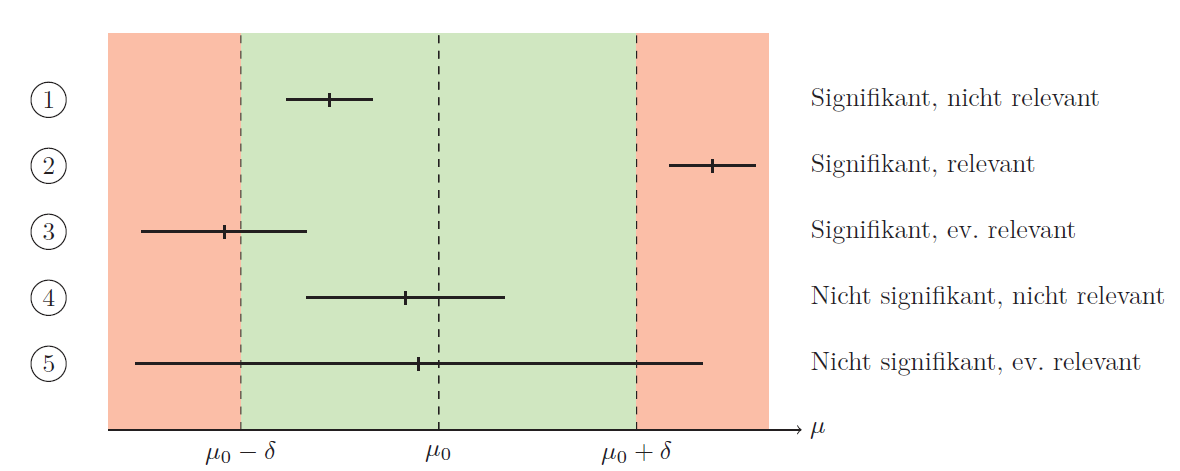
\includegraphics[width=0.95\linewidth]{img/statistical-relevance}
\end{center}
The confidence intervals for $\mu$ are represented by dashes. The "irrelevant region"
spans from $\mu_0 - \delta$ to $\mu_0 + \delta$ (green). $\delta$ was specified on the basis of expert knowledge.

\section{Simple Linear Regression}
\subsection{Regression Analysis}
Regression analysis represents a statistical method to study and model the relationship between a response variable and predictor variables. Principal goal of regression analysis is to
\begin{itemize}[noitemsep]
	\item predict data points based for some new values of the predictor variables (prediction)
	\item understand how the response variable is affected by a change of the predictor variables (inference)
\end{itemize}

\begin{center}
	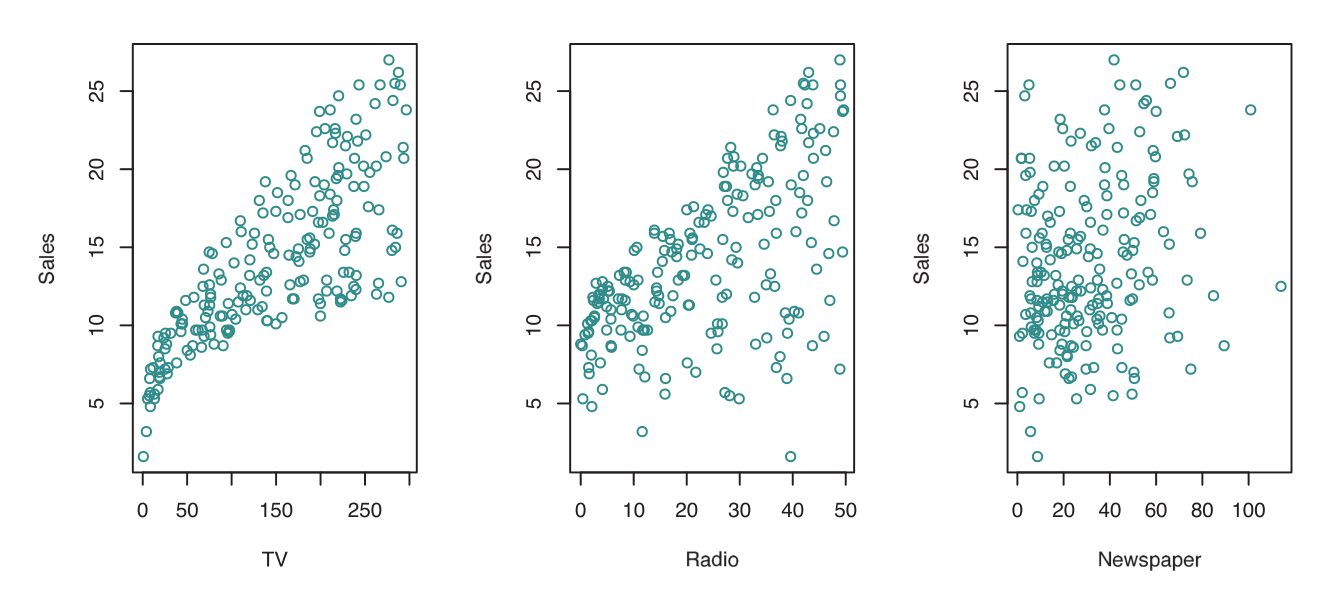
\includegraphics[width=0.8\linewidth]{img/sales_advertising}
\end{center}

The basic assumption behind this is, that there is a relationship between $Y$ and $X_1, X_2, X_3$ and deviations are random
\begin{equation*}
	Y = f(X_1, X_2,\dots, X_p) + \epsilon
\end{equation*}
\begin{itemize}
	\item $f$ is some \emph{fixed} but unknown function of $X_1, X_2,\dots, X_p$
	\item $\epsilon$ is a random error term which is independent of $X_1, X_2,\dots, X_p$ and is $\sim\N{0,r^2}$
\end{itemize}
The simple assumption is that $f$ is linear. But Linear Regression also allows to fit non-linear curves.

\subsection{Simple Linear Regression Model}
The assumption is that there is an approximately linear relationship between $X$ and $Y$
\begin{equation*}
	Y \approx \beta_0 + \beta_1 X
\end{equation*}
\begin{itemize}[noitemsep]
	\item $\beta_0$ represents the \textbf{intercept} of the regression line
	\item $\beta_1$ measures the \textbf{slope} of the regression line
	\item $\approx$ reads as "is approximately modelled as"
\end{itemize}
The coefficient estimates are denoted as $\hat{\beta}_0, \hat{\beta}_1$.

\subsection{Least Squares Method}
Let $\hat{y}_i = \hat{\beta}_0 + \hat{\beta}_1 x_i$ be the predictor for $Y$ based on the $i$th value of $X$. The $i$th residual is thus $r_i = y_i - \hat{y}_i$ and stands for the difference between the $i$th observed response value and the $i$th predicted response value of the model. The Least Squares approach chooses $\hat{\beta}_0$ and $\hat{\beta}_1$ to minimise the residual sum of squares
\begin{equation*}
	\text{RSS} = r_1^2 + r_2^2 + r_3^2 + \dots + r_n^2
\end{equation*}

\begin{definition}
	Least Squares Coefficient Estimates
	\begin{equation*}
		\hat{\beta}_1 = \frac{\sum_{i=1}^{n}(x_i - \samplemean{x})(y_i - \samplemean{y})}{\sum_{i=1}^{n}(x_i - \samplemean{x})^2}
	\end{equation*}
	\begin{equation*}
		\hat{\beta}_0 = \samplemean{y} - \hat{\beta}_1 \samplemean{x}
	\end{equation*}
	where
	\begin{equation*}
		\samplemean{x} = \frac{1}{n}\sum_{i=1}^{n} x_i\qquad\text{and}\qquad\samplemean{y} = \frac{1}{n}\sum_{i=1}^{n} y_i	
	\end{equation*}
\end{definition}

\begin{definition}
	Standard Error
	\begin{equation*}
		\text{se}(\hat{\beta}_0)^2 = \sigma^2 \left( \frac{1}{n} + \frac{\samplemean{x}^2}{\sum_{i=1}^{n}(x_i - \samplemean{x})^2} \right) \qquad\text{and}\qquad \text{se}(\hat{\beta}_1)^2 = \frac{\sigma^2}{\sum_{i=1}^{n}(x_i-\samplemean{x})^2}
	\end{equation*}
	where $\sigma^2 = \Var{\epsilon}$
\end{definition}
In general $\sigma^2$ (the variance of the error term) is not known, but can be estimated on the basis of the data.
\begin{equation*}
	\hat{\sigma} = \text{RSE} = \sqrt{\frac{\text{RSS}}{n-2}} = \sqrt{\frac{r_1^2 + r_2^2 + \dots + r_n^2}{n-2}}
\end{equation*}
The factor $\frac{1}{n-1}$ is chosen so that the estimate of $\sigma$ turns out \textbf{unbiased}.

\subsection{Hypothesis Test}
\begin{itemize}[noitemsep]
	\item $H_0$ There is \textbf{no} relationship between $X$ and $Y$, \quad $\beta_1 = 0$
	\item $H_A$ There is \textbf{some} relationship between $X$ and $Y$, \quad $\beta_1 \neq 0$
\end{itemize}
To test this hypothesis, it must be determined whether $\beta_1$ is sufficiently far from zero that there is confidence that $\beta_1$ is non-zero.

\subsection{The Test Statistic T}
\begin{definition}
	A 95\% confidence interval is defined as a range of values such that with a 95\% probability, the range will contain the true unknown parameter. The range is defined in terms of lower and upper limits computed from the sample of data.
\end{definition}
The 95\% confidence can be calculated by
\begin{equation*}
	\left[ \hat{\beta}_1 - t_{0.975, n-2} \cdot \text{se}(\hat{\beta}_1), \hat{\beta}_1 + t_{0.975, n-2} \cdot \text{se}(\hat{\beta}_1) \right]
\end{equation*}

\subsection{Prediction Interval}
An important task in statistics consists of predicting future observations $Y$ for a given value of $X$. Usually the variability of the fitted value $\widehat{Y}$ is not interesting, but the variability of the future observation is. This variability is called prediction interval.

There might be the temptation to use the confidence interval to indicate the interval twidehat contains a future observation for a given $x_0$. However, this interval contains the expected value of $\widehat{y}_0 = \widehat{\beta}_0 + \widehat{\beta}_1 x_0$ only with a given probability. The scatter around the regression line expressed by the error term $\epsilon$ has to be accounted for as well. Thus the prediction interval can be calculated as follows
\begin{equation*}
	\text{se}(y_0)^2 = \widehat{\sigma}^2\left(1 + \frac{1}{n} + \frac{(x_0 - \samplemean{x})^2}{\sum_{i=1}^{n}(x_i - \samplemean{x})^2}\right)
\end{equation*}

\subsection{Model Assumptions for the Error Terms $\epsilon_i$}
All test and estimation methods rely on model assumptions that the error terms $\epsilon_i$ are independent and normally distributed random variables with a constant variance
\begin{equation*}
	\epsilon_i \quad \text{i.i.d.} \quad \N{0,\sigma^2}
\end{equation*}
The error term $\epsilon_i = y_i - \left( \beta_0 + \beta_1 x_i \right)$ since $\beta_0$ and $\beta_1$ are unknown. However, the residuals $r_i = y_i - \left( \hat{\beta}_0 + \hat{\beta}_1 x_i \right)$ can be determined and are relevant to estimate the standard deviation of the error terms.

\subsubsection{Residual Standard Error}
The RSE is an estimate of the standard deviation of $\epsilon$. Roughly speaking, it is the average amount that the response will deviate from the true regression line.
\begin{equation*}
	\text{RSE} = \sqrt{\frac{r_1^2 + \dots + r_n^2}{n-2}} = \sqrt{\frac{(y_1 - \hat{y}_1)^2 + \dots + (y_n - \hat{y}_n)^2}{n-2}}
\end{equation*}
\begin{equation*}
	r = \Cor{X,Y} = \frac{\sum_{i=1}^{n}(x_i - \samplemean{x})(y_i - \samplemean{y})}{\sqrt{\sum_{i=1}^{n} (x_i - \samplemean{x})}\sqrt{\sum_{i=1}^{n} (y_i - \samplemean{y})}}
\end{equation*}

\subsection{Diagnostic Tool for Testing Model Assumptions}
To identify a non-linearity of regression function $f$, that is to falsify the model assumption $\ev{\epsilon_i} = 0$, the Tukey-Anscombe-Plot can be used.\\
\paragraph{Tukey-Anscombe-Plot}
\begin{itemize}
	\item Plot the residuals $r_i = y_i - \hat{y}_i$ on the vertival axis
	\item Plot the fitted or predicted values $\hat{y}_i$ on the horizontal axis
\end{itemize}
The expectation is that the LOESS smoother is linear around 0.
\begin{center}
	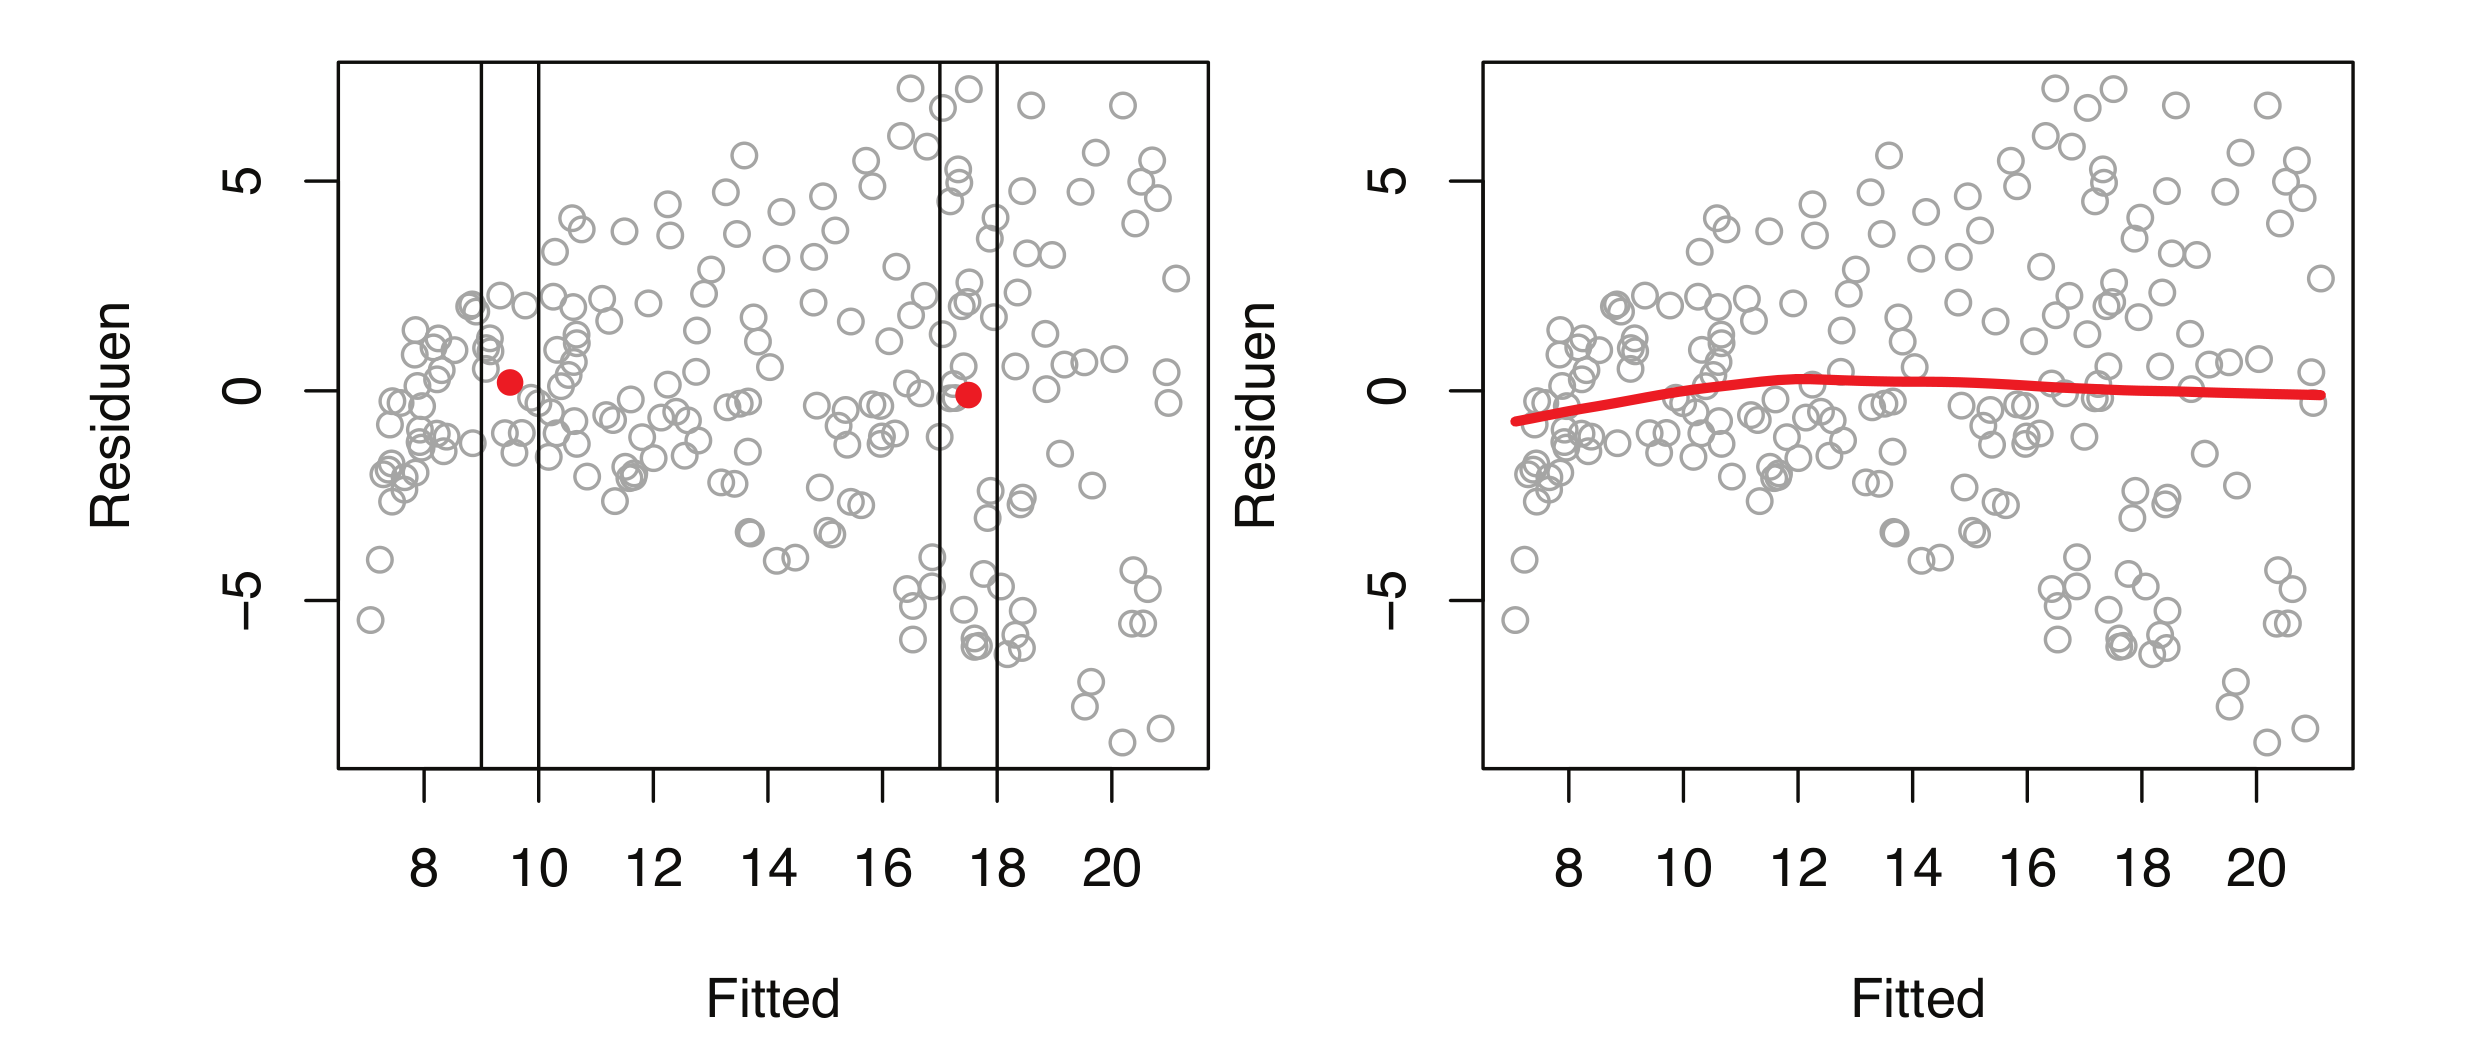
\includegraphics[width=0.8\linewidth]{img/LOESS_smoother}
\end{center}
To identify a non-constant variance in the error terms $\epsilon_i$ the standardized residuals are used
\begin{equation*}
	\tilde{r}_i = \frac{r_i}{\hat{\sigma}\sqrt{1 - \left( \frac{1}{n} + \frac{(x_i - \samplemean{x})^2}{\sum_{j=1}^{n}(x_j - \samplemean{x})^2} \right)}}
\end{equation*}
With $\hat{\sigma}$ being the estimate of the standard deviation of the error terms, and estimated by the residual standard error. If the error terms are normally distributed then $\tilde{r}_i \sim \N{0,1}$.

The resulting standardized residuals are then plotted in a so-called QQ-plot
\begin{center}
	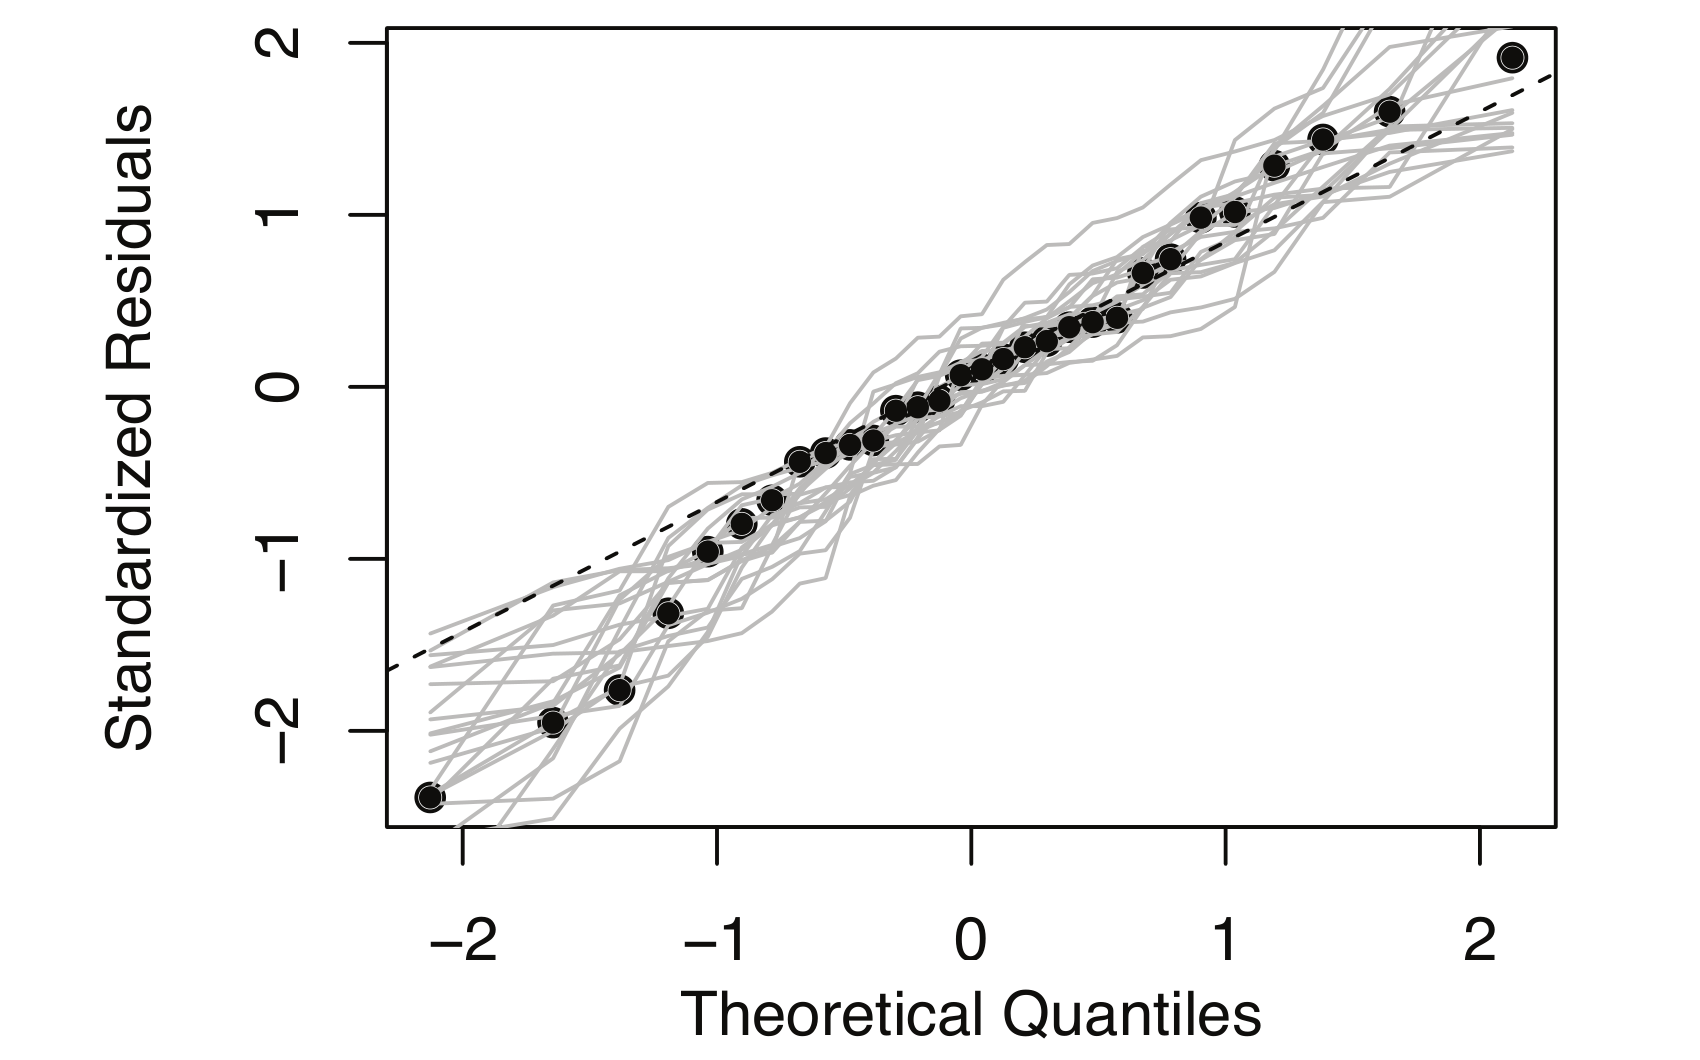
\includegraphics[width=0.5\linewidth]{img/QQ_plot}
\end{center}
\begin{theorem}
	The consequences for case of correlated error terms is that the  the estimated standard errors will tend to underestimate the true standard errors. As a result, confidence and prediction intervals will be narrower than they should be.
\end{theorem}

\subsection{Outliers}
An outlier is point for which $y_i$ is far from value $\hat{y}_i$ predicted by model. A leverage point is a point with an unusual value for $x_i$ and can be identified by the \textbf{leverage statistic}
\begin{equation*}
	h_i = \frac{1}{n} + \frac{(x_i + \samplemean{x})^2}{\sum_{i' = 1}^{n}(x_{i'}-\samplemean{x})^2}
\end{equation*}
While the Cook's distance measures the influence of an observation
\begin{equation*}
	d_i = \frac{1}{\hat{\sigma}^2}\cdot\left(\underline{\hat{y}}_{(-i)} - \underline{\hat{y}}\right)^T \left(\underline{\hat{y}}_{(-i)} - \underline{\hat{y}}\right) = \tilde{r}_i^2 \frac{h_i}{2(1-h_i)}
\end{equation*}
The larger the value of Cook’s distance $d_i$ is, the higher is the influence of the corresponding observation on the estimation of the predicted value $\hat{y}_i$. An observation with a value of Cook’s distance larger than 1 is considered as dangerously influential.











\newpage
\newpage
\section{Multivariate Probability Distributions}

\subsection{Discrete Joint Probability Distributions}
The joint distribution of two discrete random variables $X$ and $Y$, having their values in $W_X$ and in $W_Y$ respectively, is defined by the joint probability distribution of $X$ and $Y$, that is by the following probabilities
\begin{equation*}
	P(X=x, Y=y), x\in W_X, y\in W_Y
\end{equation*}
Single distributions $P(X = x)$ of $X$ and $P(Y = y)$ of $Y$ are called marginal distributions of the joint random variable $(X,Y)$. Marginal distributions can be calculated based on their joint distribution
\begin{equation*}
	P(X=x) = \sum_{y\in W_Y} P(X = x, Y = y),\qquad x\in W_X
\end{equation*}
The conditional probability of $X$ given $Y=y$ is defined as
\begin{equation*}
	P(X = x | Y = y) = \frac{P(X = x, Y = y)}{P(Y=y)}
\end{equation*}
The marginal distributions can then be expressed as follows
\begin{equation*}
	P(X=x) = \sum_{y\in W_y} P(X=x|Y=y)P(Y=y),\qquad x\in W_X
\end{equation*}
The conditional expected value of $Y$ given $X=x$ is defined as
\begin{equation*}
	\ev{Y|X=x} = \sum_{y\in W_Y} y\cdot P(Y=y|X=x)
\end{equation*}

\subsection{Joint Probability Density}
The probability that the joint random variable $(X,Y)$ lies in a two-dimensional region $A$, that is $A\subset \R^2$, is given by
\begin{equation*}
	P\left( (X,Y) \in A \right) = \iint_{A} f_{X,Y}(x,y) \diff x \diff y
\end{equation*}
This integral corresponds to the volume enclosed by by the surface of the joint density function $f_{X,Y}(x,y)$ and by the region $A$, in particular $\iint_{\R^2} f_{X,Y}(x,y) \diff x\diff y = 1$

\subsubsection{Life Expectancy of Two Machines Example}
Consider two machines with exponentially distributed life expectancy $X\sim \Exp{\lambda_1}$ and $Y\sim\Exp{\lambda_2}$, where $X$ and $Y$ are independent random variables. What is the probability that machine one runs longer than machine two?

The density functions for life expectancy of the two machines are:
\begin{equation*}
	f_X(x) = \lambda_1 e^{-\lambda_1 x}\ \text{and}\ f_Y(y) = \lambda_2 e^{-\lambda_2 y}
\end{equation*}
Due to \textbf{independence} of the two random variables, the \textbf{joint density} can be calculated as follows
\begin{align}
	f_{X,Y} (x,y) &= f_X(x) \cdot f_Y(y)\\
	&= \lambda_1 e^{-y\lambda_1} \cdot \lambda_2 e^{-\lambda_2 y}
\end{align}
\begin{minipage}{0.6\linewidth}
	Relevant Set:
	\begin{equation*}
		A = \{(x,y)|0\leq y\leq x\}
	\end{equation*}
\end{minipage}
\begin{minipage}{0.4\linewidth}
	\begin{center}
		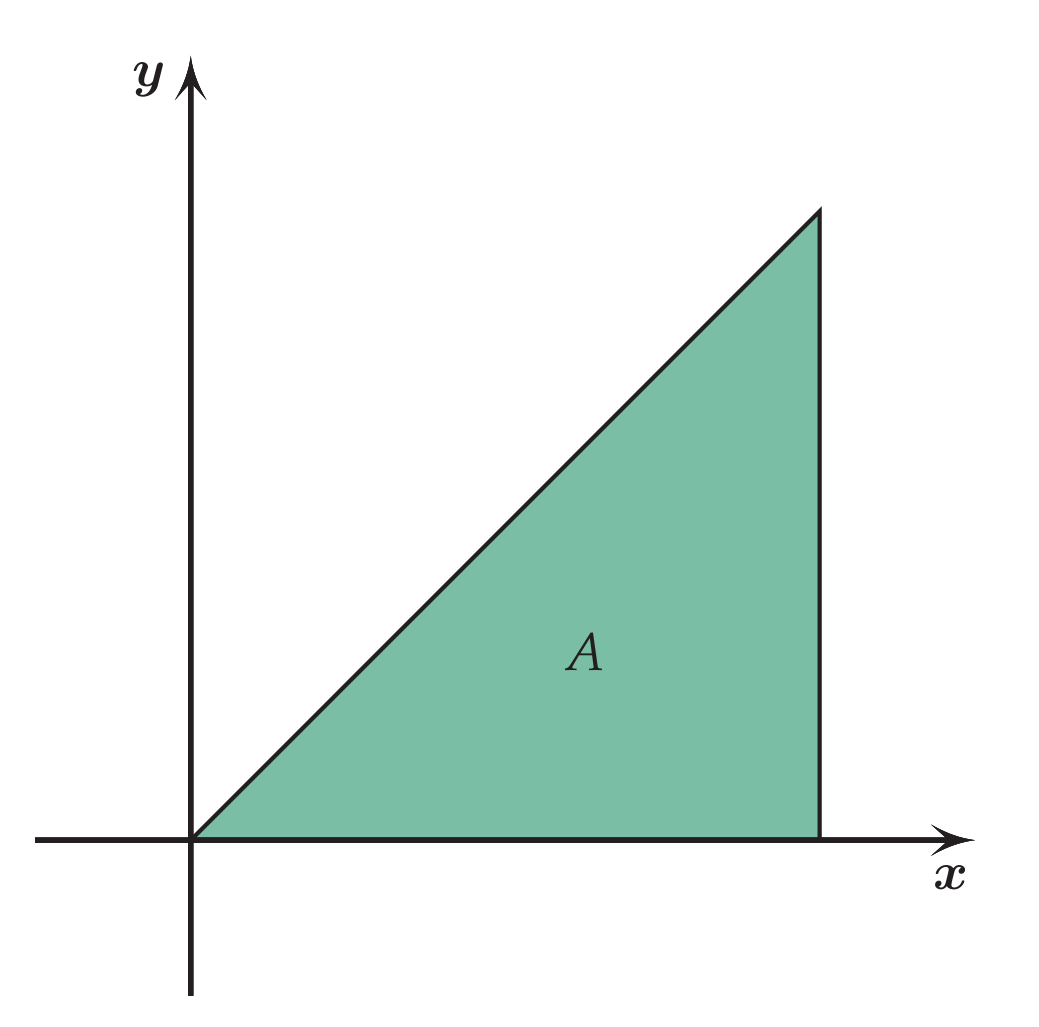
\includegraphics[width=0.6\linewidth]{img/area_A_under_xy}
	\end{center}	
\end{minipage}
Probability that machine one runs longer than machine two:
\begin{align*}
	P(Y<X) &= \int_{0}^{\infty}(\int_{0}^{x} \lambda_1 e^{-y\lambda_1} \cdot \lambda_2 e^{-\lambda_2 y} \diff y )\diff x\\
	&= \int_{0}^{\infty} \lambda_1e^{-\lambda_1 x} (1 - e^{-\lambda_2 x})\diff x\\
	&= \frac{\lambda_2}{\lambda_1 + \lambda_2}
\end{align*}

\begin{center}
	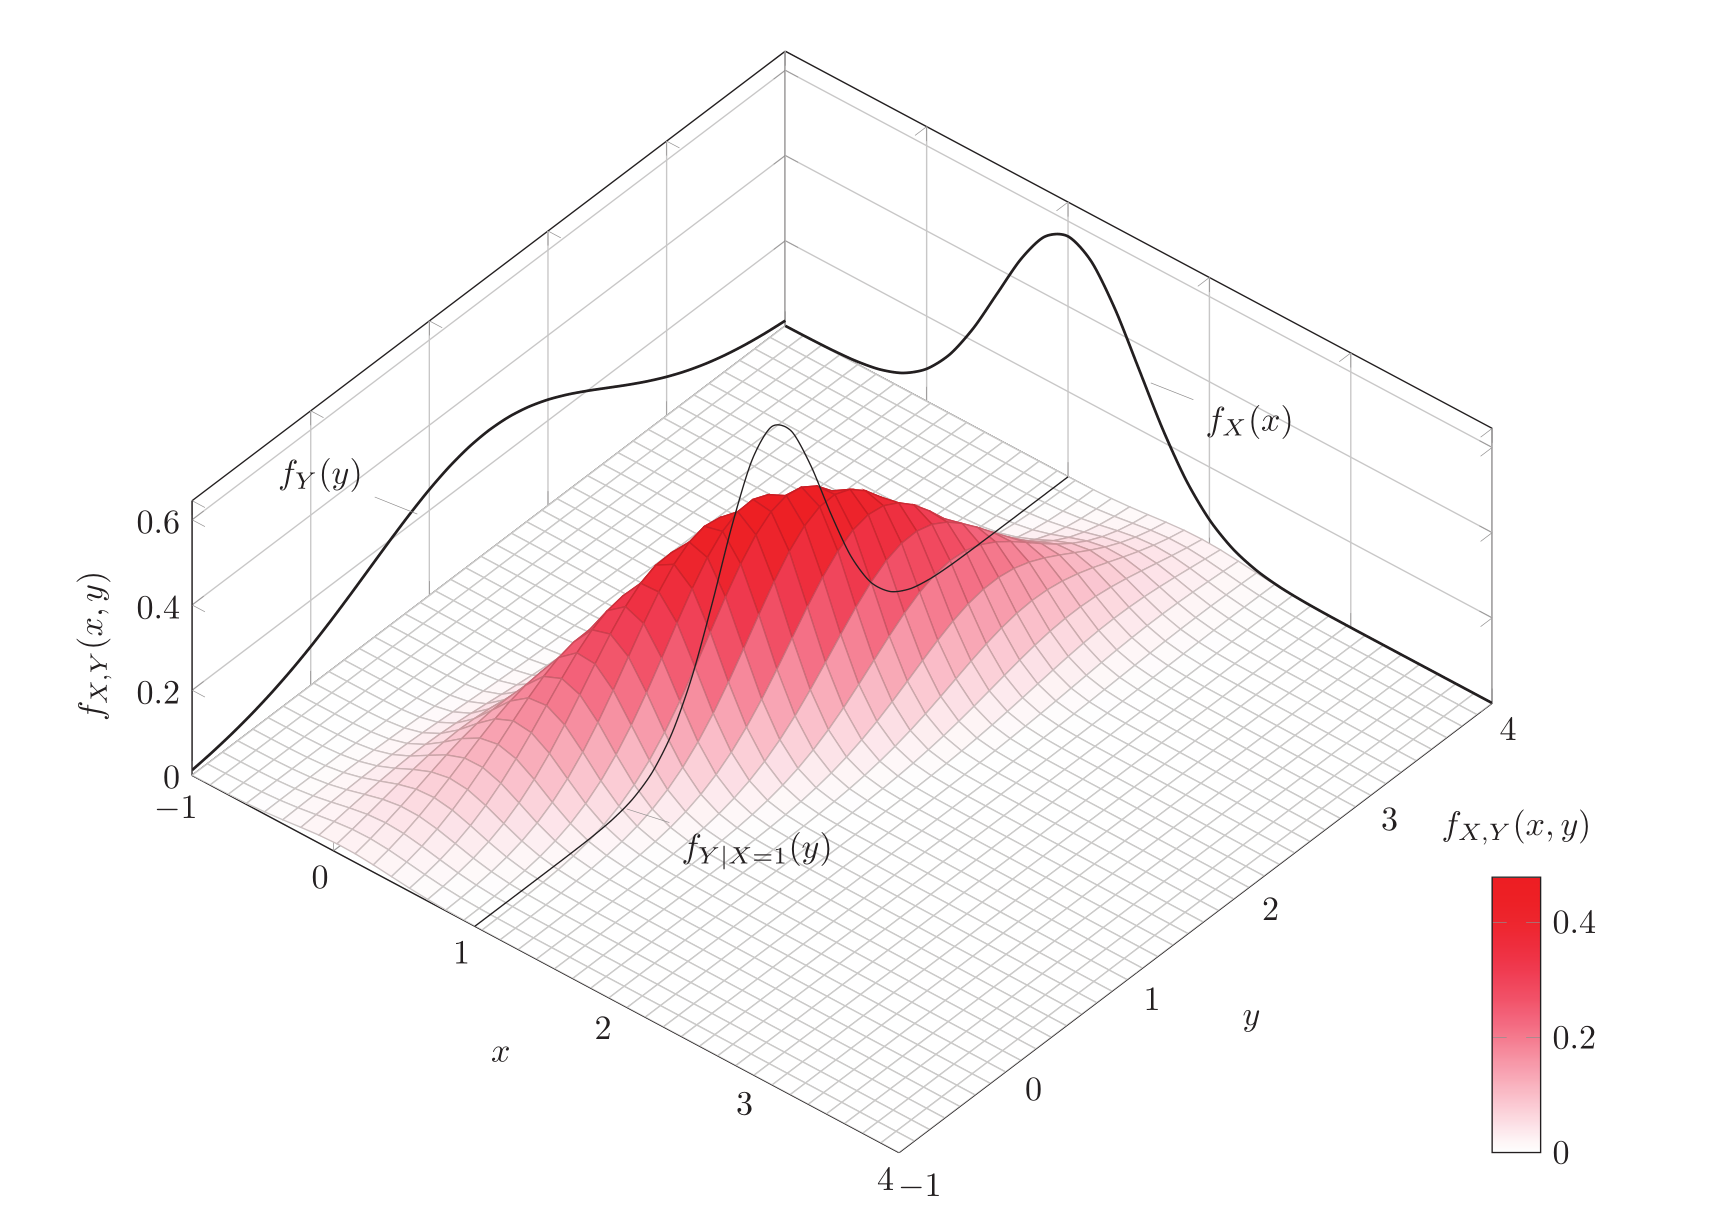
\includegraphics[width=0.8\linewidth]{img/marginal_density_xy}
\end{center}

Using the joint density, the marginal densities of $X$ and of $Y$ are obtained by integrating over the other variable
\begin{equation*}
	f_X(x) = \int_{-\infty}^{\infty}f_{X,Y}(x,y)\diff y \qquad\qquad f_Y(y) = \int_{-\infty}^{\infty}f_{X,Y}(x,y)\diff x
\end{equation*}

\begin{center}
	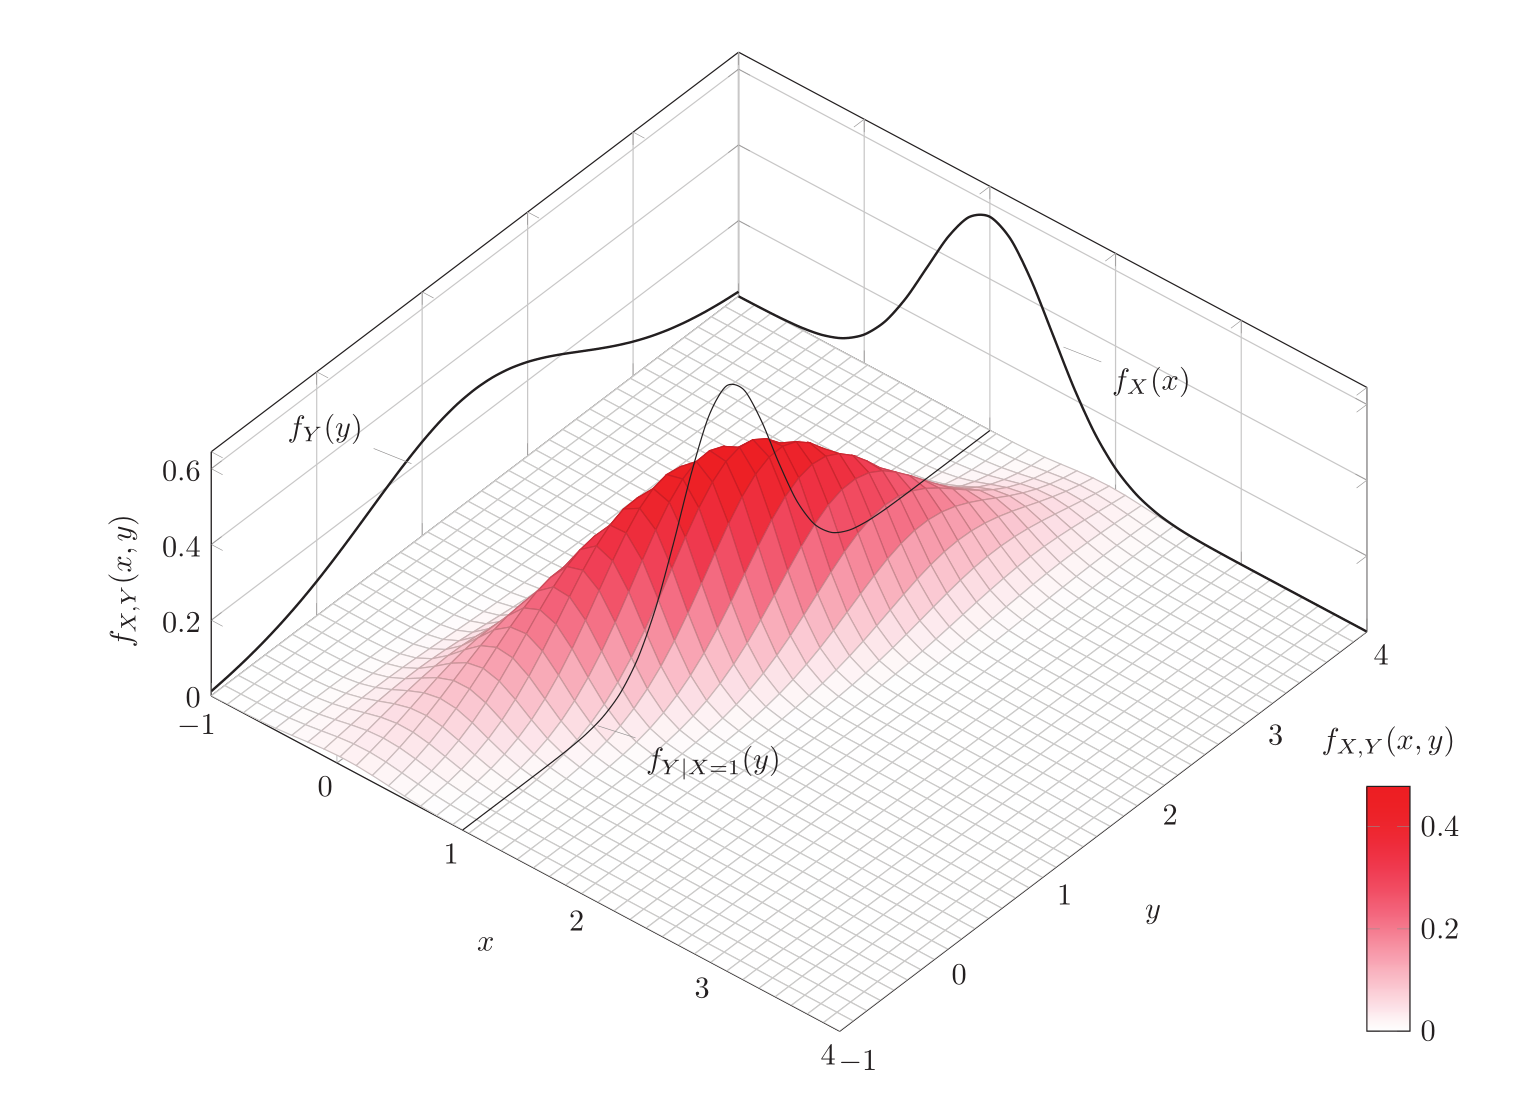
\includegraphics[width=0.8\linewidth]{img/conditional_probability_xy}
\end{center}

The conditional probability of $Y$ given $X = x$ is defined as
\begin{equation*}
	f_{(Y | X=x)} = f_Y (y | X=x) = \frac{f_{X,Y}(x,y)}{f_X(x)}
\end{equation*}
Conditional probability density corresponds to \textbf{longitudinal section} of the joint density

\subsection{Covariance and Correlation}

\subsubsection{Empirical Covariance}
\begin{minipage}{0.4\linewidth}
	\begin{center}
		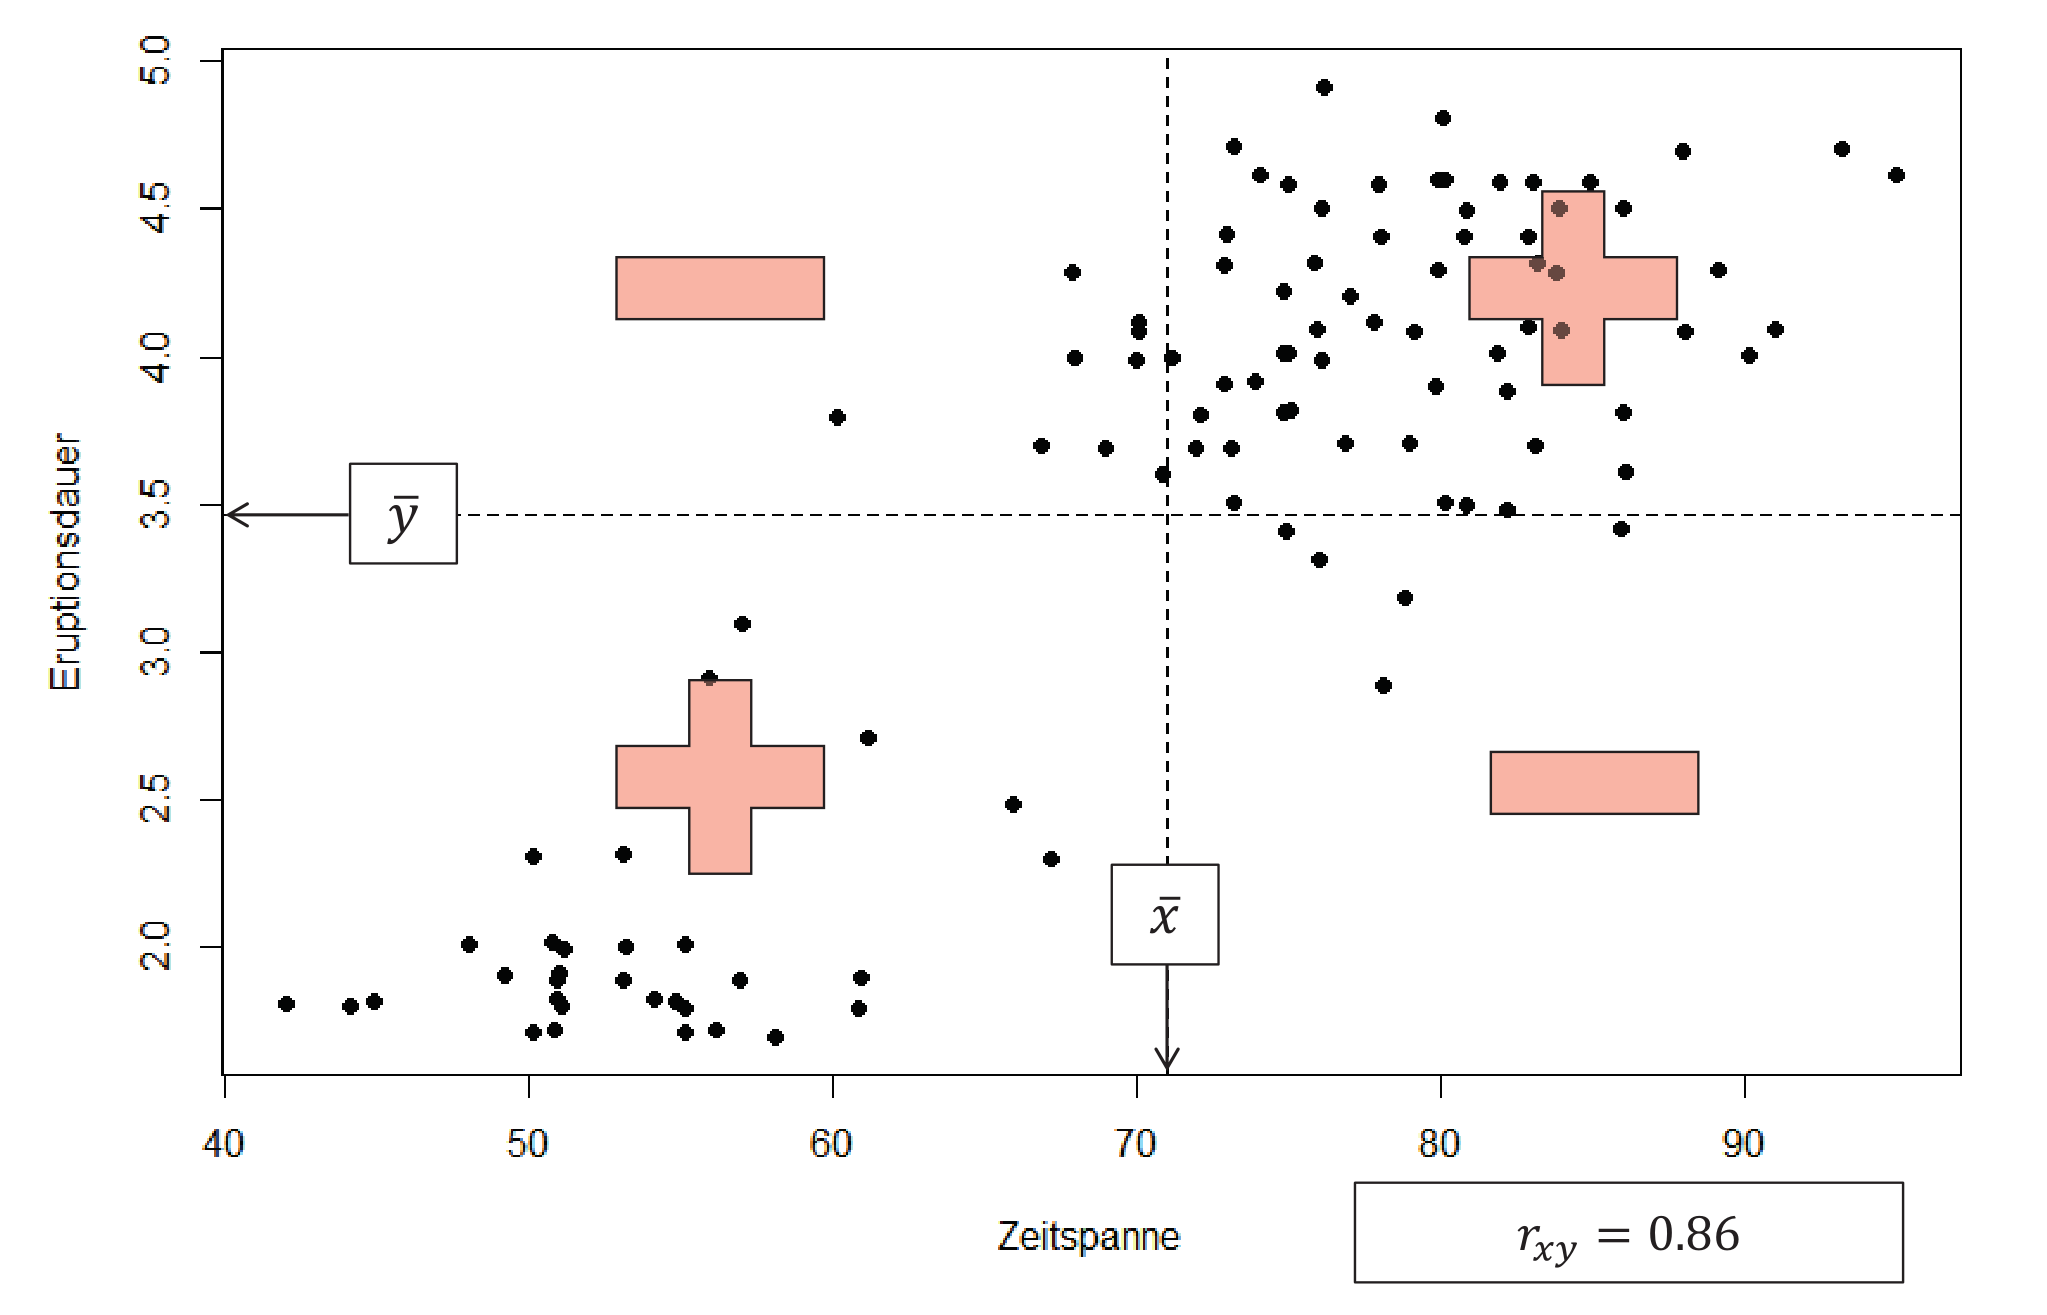
\includegraphics[width=0.9\linewidth]{img/empirical_covariance}
	\end{center}
\end{minipage}
\begin{minipage}{0.6\linewidth}
	The empirical covariance is the average value of the product of the deviation of $x_i$ from its mean $\samplemean{x}$ and the deviation of $y_i$ from its mean $\samplemean{y}$
	\begin{equation*}
		q_{xy} = \frac{1}{n-1}\sum_{i=1}^{n}(x_i - \samplemean{x} )(y-\samplemean{y})
	\end{equation*}
\end{minipage}

\subsubsection{Theoretical Covariance}
\begin{definition}
	The \textbf{covariance} of two random variables $X$ and $Y$ is defined as
	\begin{equation*}
		\Cov{X,Y} = \ev{(X-\mu_x)(Y-\mu_y)}
	\end{equation*}
\end{definition}
The covariance is the average value of the product of the deviation of $X$ from its mean $\mu_X$ and the deviation of $Y$ from its mean $\mu_Y$. If $X$ and $Y$ are \textbf{positively} associated, that is when $X$ is larger than its mean Y tends to be larger than its mean as well, the \textbf{covariance} will be \textbf{positive}. If the association between $X$ and $Y$ is \textbf{negative}, that is when $X$ is larger than its mean $Y$ tends to be smaller than its mean, the \textbf{covariance} is \textbf{negative}.

\subsection{Correlation}
\begin{definition}
	The correlation of $X$ and $Y$, denoted by $\rho$ is
	\begin{equation*}
		\Cor{X,Y} = \rho_{XY} = \frac{\Cov{X,Y}}{\sigma_X\sigma_Y}
	\end{equation*}
\end{definition}
Correlation is simply a standardized version of the covariance. Contrary to the covariance, the correlation is thus a dimensionless quantity. 

\subsubsection{Properties of the Correlation}
$\rho$ has the following property
\begin{equation*}
	-1 \leq \Cor{X,Y} \leq 1
\end{equation*}
The correlation is a measure for the strength and direction of the linear dependency between $X$ and $Y$.
\begin{align*}
	\Cor{X,Y} &= +1 \qquad\text{iff}\qquad Y=a+bX\ \text{for $a\in\R$ and $b>0$}\\
	\Cor{X,Y} &= -1 \qquad\text{iff}\qquad Y=a+bX\ \text{for $a\in\R$ and $b<0$}\\
\end{align*}
If $\abs{\Cor{X,Y}} = 1$, then there is a perfectly linear relationship between $X$ and $Y$.

\begin{definition}
	If $\Cor{X,Y}=0$ then $X$ and $Y$ are \textbf{uncorrelated}. In this case there is no linear relationship between $X$ and $Y$. There may be a non-linear relationship however.
\end{definition}

\subsubsection{Uncorrelatedness and Independence}
\begin{equation*}
	X\ \text{and}\ Y\ \text{independent} \Rightarrow \Cor{X,Y}=0\Rightarrow \Cov{X,Y}=0
\end{equation*}
However, the converse is generally not true, that is independence does not follow from uncorrelatedness.

\vspace{1em}
\noindent
These relations follow immediately from the definition of the covariance
\begin{enumerate}
	\item $\Var{X} = \Cov{X,X}$
	\item $\Cov{X,Y} = \ev{XY} - \ev{X}\ev{Y}$
	\item $\ev{XY} = \ev{X}\ev{Y}\qquad (X,Y\ \text{independent})$
	\item
	\begin{equation*}
		\Var{\sum_{i=1}^{n}X_i} = \sum_{i=1}^{n}\Var{X_i} + 2\sum_{i<j}^{n}\Cov{X_i,X_j}
	\end{equation*}
	in particular in the case of two random variables
	\begin{equation*}
		\Var{X + Y} = \Cov{X + Y, X + Y} = \Var{X} + \Var{Y} + 2\Cov{X,Y}
	\end{equation*}
	\item For $X_1,\dots,X_2$ independent:
	\begin{equation*}
		\Var{X_1+\dots+X_n} = \Var{X_1} + \dots + \Var{X_n}
	\end{equation*}
\end{enumerate}

\subsection{Bivariate Normal Distribution}
The bivariate normal distribution is completely defined by expected values and variances of the marginal distributions $\mu_X, \sigma_X^2, \mu_Y, \sigma_Y^2$ and the covariance between $X$ and $Y$, $\Cov{X,Y} = \rho_{XY}\sigma_X\sigma_Y$. The \textbf{joint density} of a bivariate normal distribution is given by
\begin{equation*}
	F_{X,Y}(x,y) = \frac{1}{2\pi\sqrt{\det(\Sigma)}} e^{-\frac{1}{2} (x-\mu_X, y-\mu_Y) \Sigma^{-1}\begin{pmatrix}
		x-\mu_X\\
		y-\mu_Y
		\end{pmatrix} }
\end{equation*}
and the \textbf{covariance matrix} $\Sigma$ is defined as
\begin{equation*}
	\Sigma = \begin{pmatrix}
	\Cov{X,X} & \Cov{X,Y}\\
	\Cov{X,Y} & \Cov{Y,Y}
	\end{pmatrix}
	=
	\begin{pmatrix}
		\sigma_X^2 & \rho_{XY}\sigma_X\sigma_Y\\
		\rho_{XY}\sigma_X\sigma_Y & \sigma_Y^2
	\end{pmatrix}
\end{equation*}
The \textbf{marginal distributions} of bivariate normal distributions are again normal distributions
\begin{equation*}
	X\sim\N{\mu_X,\sigma_X^2}\qquad\text{and}\qquad Y\sim\N{\mu_Y,\sigma_Y^2}
\end{equation*}
The correlation between $X$ and $Y$ is given by the predefined value $\rho_{XY}$, for example $\rho_{XY} = -0.85$. Contour lines of the bivariate normal distribution are \textbf{ellipses}. The higher the absolute value of the correlation $\rho_{XY}$, the narrower the ellipses are (see figure \ref{fig:correlationcontourlines}).

\begin{figure}[tbh]
	\centering
	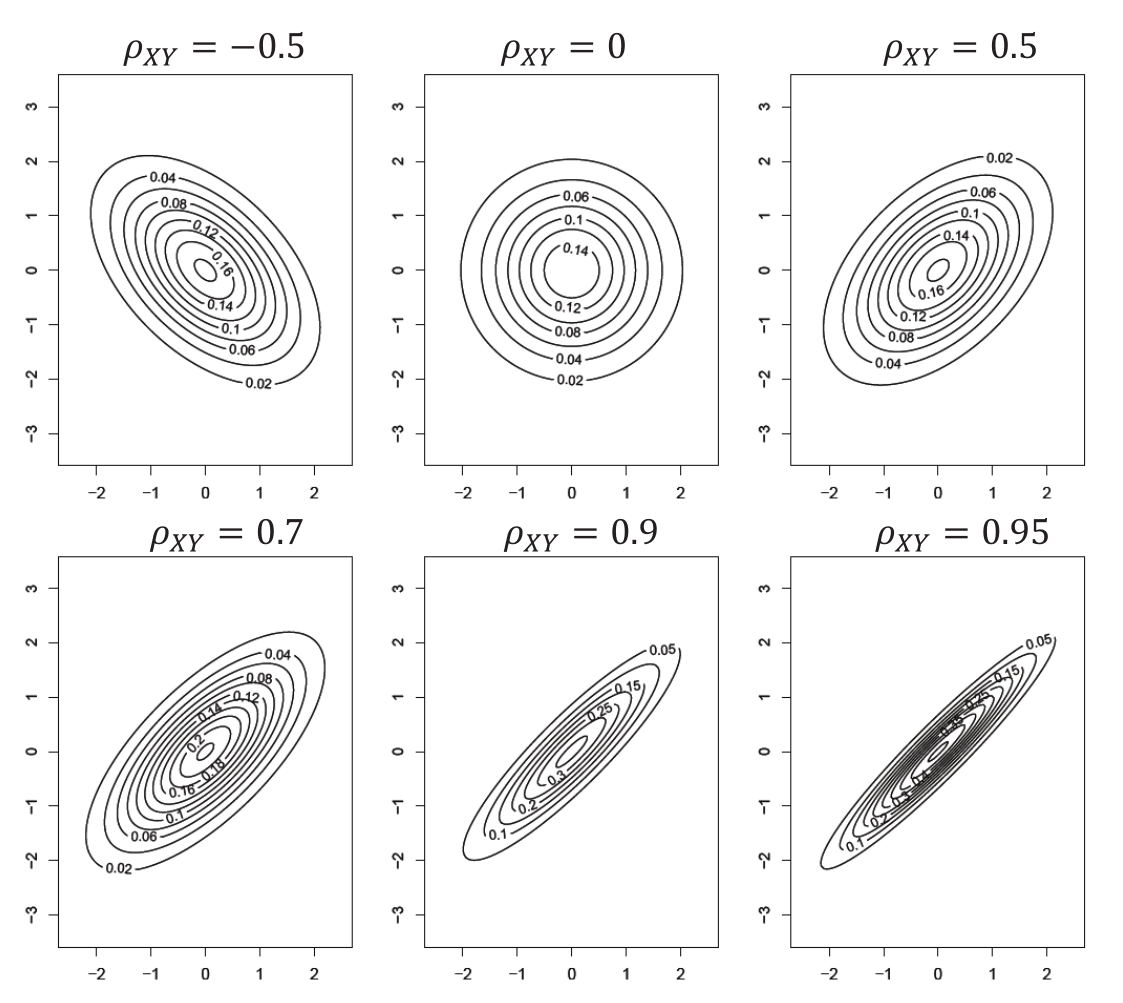
\includegraphics[width=0.6\linewidth]{img/correlation_contour_lines}
	\caption{Contour lines of bivariate normal distributions for different correlation coefficients}
	\label{fig:correlationcontourlines}
\end{figure}

\subsection{Principal Component Analysis}
Principal component analysis is a popular approach for deriving a low-dimensional set of features from a large set of variables.
PCA is a technique for \textbf{reducing} the dimension of a $n \times p$ data matrix $X$ where $n$ corresponds to the number of observations and $p$ to the number of variables.
\textbf{First principal component} direction of the data is that along which the observations \textbf{vary the most}.

\begin{figure}[H]
	\centering
	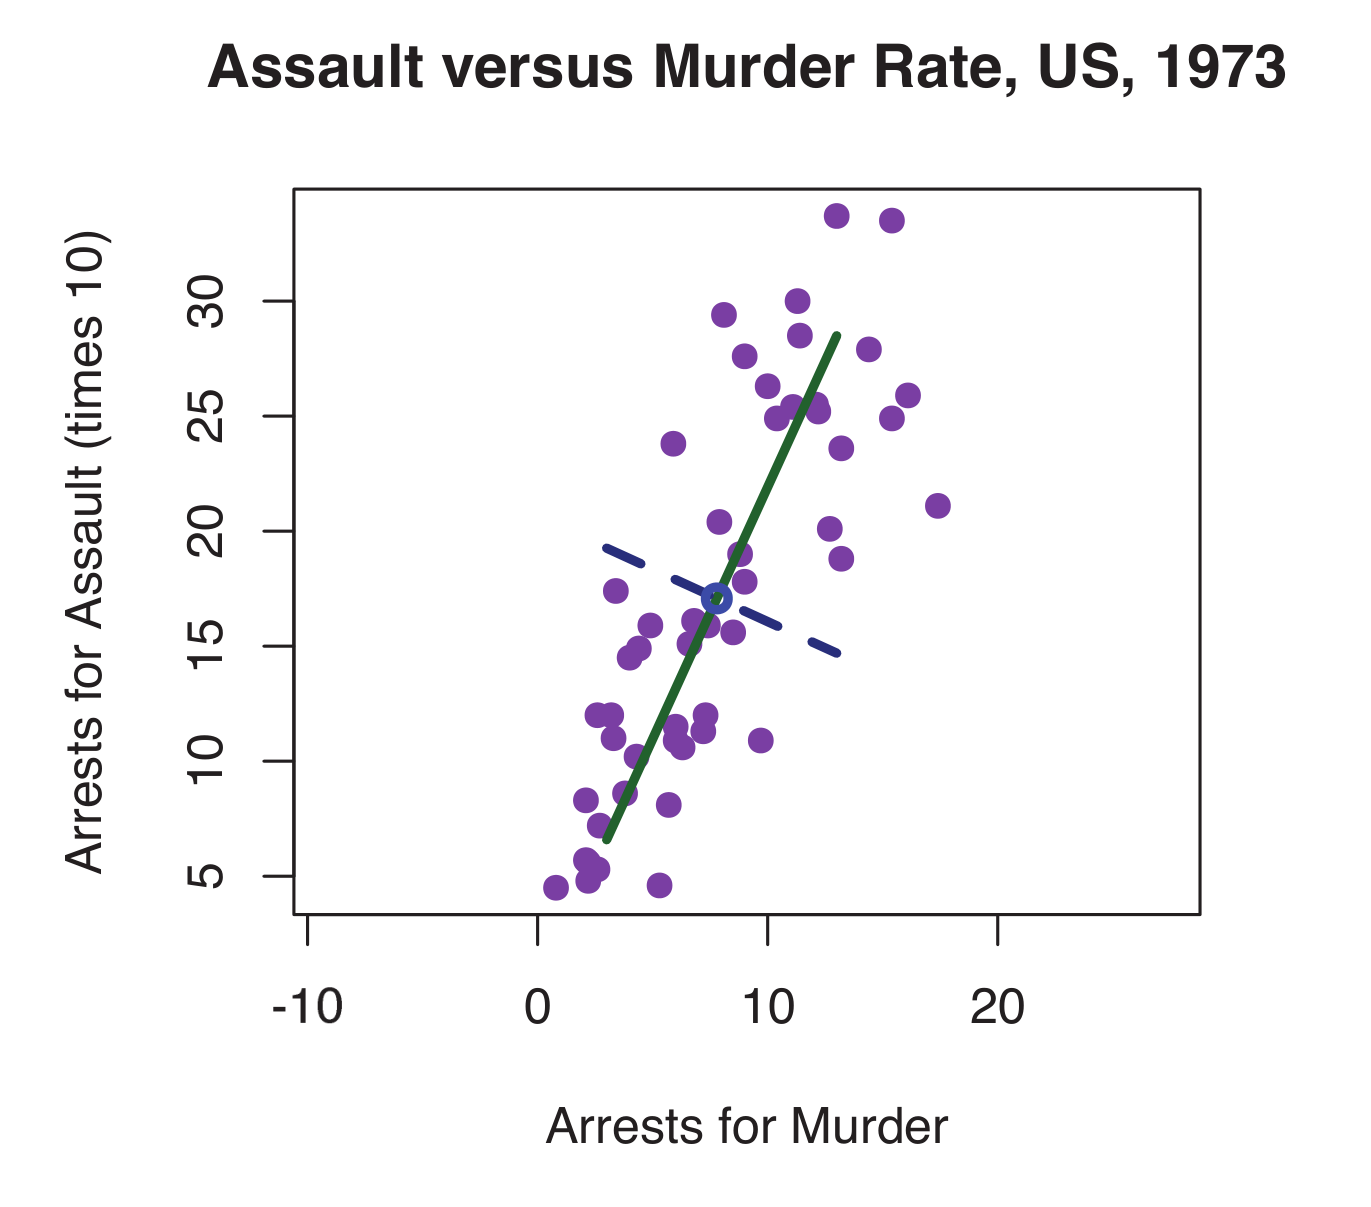
\includegraphics[width=0.6\linewidth]{img/Principal_component_analysis}
	\caption{Principal component decomposition of the \predvar{USArrests} dataset}
	\label{fig:principalcomponentanalysis}
\end{figure}

The green solid line in figure \ref{fig:principalcomponentanalysis} \textbf{represents the first principal component direction} of the data which is the direction along which there is the greatest variability in the data.

The projection of the observations onto this \textbf{ first principal component direction} results in the projected observations having the largest possible variance.

\begin{figure}[H]
	\centering
	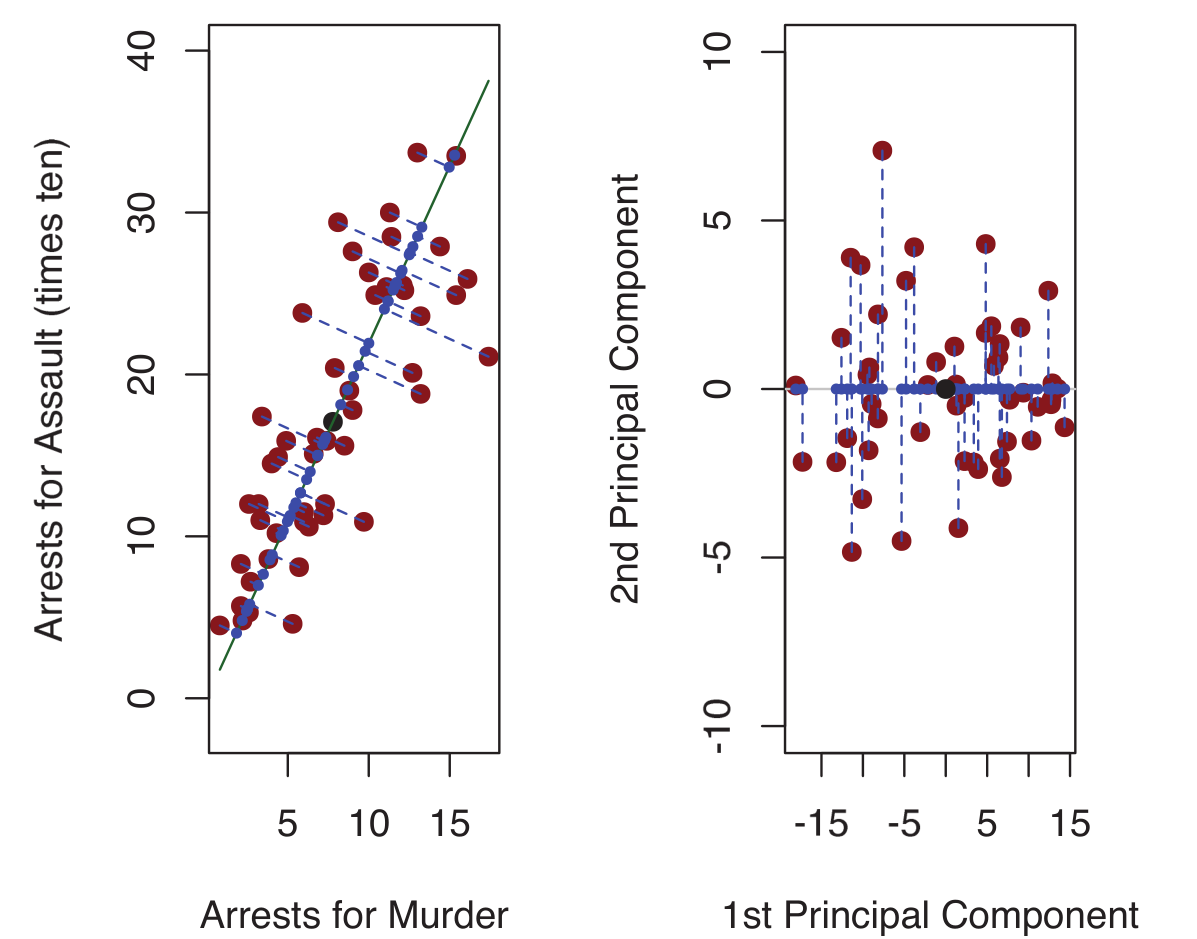
\includegraphics[width=0.6\linewidth]{img/Principal_component_analysis02}
	\caption{Projection on the first principal component direction}
	\label{fig:principalcomponentanalysis02}
\end{figure}

The two principal components $Z_1$ and $Z_2$ are \textbf{uncorrelated}, which implies that their covariance matrix $\Sigma$ has vanishing off-diagonal elements. Thus the covariance matrix has to be diagonalised by transforming the basis vectors. This can be achieved by an appropriate rotation matrix $\Phi$ so that
\begin{align*}
\begin{pmatrix} Z_1\\Z_2 \end{pmatrix} = (X-\mu_X, Y-\mu_Y) \cdot \begin{pmatrix}\phi_{11}&\phi_{12}\\\phi_{21}&\phi_{22}\end{pmatrix} &= \begin{pmatrix}
\phi_{11}(X-\mu_X) + \phi_{21}(Y-\mu_Y)\\
\phi_{12}(X-\mu_X) + \phi_{22}(Y-\mu_Y)
\end{pmatrix}\\
\intertext{and}
\begin{pmatrix} \Cov{Z_1,Z_1} & \Cov{Z_1,Z_2}\\ \Cov{Z_2,Z_1} & \Cov{Z_2,Z_2} \end{pmatrix} &= \begin{pmatrix} \sigma_{Z_1}^2 & 0 \\ 0 & \sigma_{Z_2}^2 \end{pmatrix}
\end{align*}
The rotation matrix $\Phi$ needs to satisfy the condition $\phi_{11}^2 + \phi_{21}^2 = 1$ and $\phi_{12}^2 + \phi_{22}^2 = 1$

\vspace{1em}
\noindent
For the example dataset \predvar{USArrests} the PCA is done with
\begin{minted}{R}
pr.out <- prcomp(USArrests[, c("Murder", "Assault")])
head(pr.out$x)

## PC1 PC2
## Alabama -65.40950 2.6728663
## Alaska -92.25166 -1.6559620
## Arizona -123.14478 -4.8535831
## Arkansas -19.26551 0.2047123
## California -105.19832 -3.1999471
## Colorado -33.21549 -1.2812733

pr.out <- prcomp(USArrests[, c("Murder", "Assault")])
pr.out$rotation[, 2]

## Murder Assault
## 0.9991213 -0.0419126
\end{minted}
If the first principal component direction is considered as a coordinate axis, then any point $(\predvar{Murder},\predvar{Assault})$ has the following first principal component coordinate when projected onto the line
\begin{equation*}
Z_1 = -0.0419126\cdot(\text{\predvar{Murder}} - \overbar{\text{\predvar{Murder}}}) - 0.9991213\cdot(\text{\predvar{Assault}} - \overbar{\text{\predvar{Assault}}})
\end{equation*}
The point $(\overbar{\text{\predvar{Murder}}},\overbar{\text{\predvar{Assault}}})$ corresponds to the origin on the first principal component axis, where $\overbar{\text{\predvar{Murder}}}$ indicates the mean of all $\predvar{Murder}$ values in this data set, and $\overbar{\text{\predvar{Assault}}}$ indicates the mean of all arrests for $\predvar{Assault}$ values.

$\phi_{11} = -0.0419126$ and $\phi_{21} = -0.9991213$ are the \textbf{principal component loadings}. They are chosen such that
\begin{equation*}
\Var{\phi_{11}\cdot(\text{\predvar{Murder}} - \overbar{\text{\predvar{Murder}}}) + \phi_{21}\cdot(\text{\predvar{Assault}} - \overbar{\text{\predvar{Assault}}})}
\end{equation*}
is \textbf{maximised} under the constraint $\phi_{11}^2 + \phi_{12}^2 = 1$.

The second principal component $Z_2$ is a linear combination of predictor variables and is uncorrelated with $Z_1$, and has largest variance subject to this constraint. The zero correlation condition of $Z_1$ with $Z_2$ is equivalent to the condition that the direction must be \textbf{perpendicular} or \textbf{orthogonal} to the first principal component direction


\section{Multiple Linear Regression, Qualitative Predictors and Interaction Effects}
\subsection{Multiple Linear Regression}
\begin{definition}
	\begin{equation*}
		Y = \beta_0 + \beta_1 X_1 + \beta_2 X_2 + \dots + \beta_p X_p + \epsilon
	\end{equation*}
	\begin{itemize}[label=]
		\item $X_j$ \quad $j$th predictor variable
		\item $\beta_j$ \quad association between $X_j$ and response variable $Y$
	\end{itemize}
\end{definition}

\subsection{Hypothesis Testing Using the F-Statistic}
Compute the F-Statistic as follows
\begin{equation*}
	F = \frac{\frac{\text{TSS} - \text{RSS}}{p}}{\frac{\text{RSS}}{n-p-1}} \qquad \text{TSS} = \sum_{i=1}^{n} (y_i - \samplemean{y})^2 \qquad \text{RSS} = \sum_{i=1}^{n} (y_i - \hat{y})^2
\end{equation*}
If the linear model assumptions are \textbf{correct}, it can be shown that
\begin{equation*}
	\ev{\frac{\text{RSS}}{n-p-1}} = \sigma^2
\end{equation*}
Provided the Null-Hypothesis is \textbf{true}, it can be shown that
\begin{equation*}
	\ev{\frac{\text{TSS}-\text{RSS}}{p}} = \sigma^2
\end{equation*}
That means that if there is \textbf{no} relationship between the response and the predictors, then the value of the F-Statistic is approximately 1.

When $H_0$ is true and the errors $\epsilon_i$ follow a normal distribution, the F-Statistic follows an F-distribution with $p$ and $n-p-1$ degrees of freedom.

If $H_A$ is \textbf{true}, then 
\begin{equation*}
	\ev{\frac{\text{TSS}-\text{RSS}}{p}} > \sigma^2
\end{equation*}
and the value of the F-Statistic is expected to be greater than 1.

\subsubsection{F-Test}
\begin{itemize}[label=]
	\item Null Hypothesis
	\begin{equation*}
		H_0:\quad \beta_1 = \beta_2 = \dots = \beta_p = 0
	\end{equation*}
	\item Alternative Hypothesis
	\begin{equation*}
		H_A:\quad \text{at least one $\beta_i$ is non-zero}
	\end{equation*}
	\item Assuming $H_0$ is true
	\begin{equation*}
	F = \frac{\frac{\text{TSS} - \text{RSS}}{p}}{\frac{\text{RSS}}{n-p-1}} \sim \F{p,n-p-1}
	\end{equation*}
\end{itemize}

\subsection{Factor Variable}
If a predictor variable has multiple levels, the variable gets split in multiple dummy variables. For example given a variable \predvar{ethnicity} with three levels, two dummy variables get introduced
\begin{align*}
	x_{i1} &= \left\{ \begin{matrix}1 & \text{if $i$th person is Asian}\\ 0 & \text{if $i$th person is not Asian}\end{matrix} \right.\\
	x_{i2} &= \left\{ \begin{matrix}1 & \text{if $i$th person is Caucasian}\\ 0 & \text{if $i$th person is not Caucasian}\end{matrix} \right.
	\intertext{\textbf{Regression Model}}
	y_{i} = \beta_0 + \beta_1 x_{i1} + \beta_2 x_{i2} + \epsilon_i &= \left\{ \begin{matrix}
	\beta_0 + \beta_1 + \epsilon_i & \text{if $i$th person is Asian}\\
	\beta_0 + \beta_2 + \epsilon_i & \text{if $i$th person is Caucasian}\\
	\beta_0 + \epsilon_i & \text{if $i$th person is Afro-American}
	\end{matrix} \right.\\
\end{align*}
The level without a dummy variable is known as the baseline. There are many different ways of coding qualitative variables, no effect on regression fit, but does alter interpretation of coefficients and p-values

\subsection{Interaction Effects}
Having an Additivity in the model means that the effect of changes in a predictor $X_j$ on the response $Y$ is independent of the values of the other predictors. If the changes on one predictor have an effect on another predictor, then there is an \textbf{interaction effect}.
\begin{equation*}
	\predvar{sales} = \beta_0 + \beta_1 \cdot \predvar{TV} + \beta_2\cdot\predvar{radio} + \beta_3\cdot(\predvar{TV}\cdot\predvar{radio}) + \epsilon
\end{equation*}
\begin{minted}{R}
Advertising <- read.csv('Advertising.csv', header=True)
summary(lm(sales ~ TV + radio + TV * radio, data = Advertising))
# equivalent
summary(lm(sales ~ TV * radio, data = Advertising))
\end{minted}

\section{Polynomial Regression, Residual Analysis and Model Selection}

\subsection{Polynomial Regression Model}

\begin{equation*}
	Y = \beta_0 + \beta_1\cdot X + \beta_2\cdot X^2 + \epsilon
\end{equation*}

\begin{minted}{R}
lm(Y ~ X + I(X^2), data = Data)
\end{minted}

\subsection{Identification of Collinearity}
Collinearity refers to the situation in which two or more predictor variables are closely related to one another. Collinearity can be detected by using the \textbf{correlation matrix} \mintinline{R}{cor(Data)} and the \textbf{variance inflation factor}
\begin{equation*}
	\text{VIF}(\hat{\beta}_j) = \frac{1}{1- R_{(X_j|X_{-j})}^2}
\end{equation*}
\begin{itemize}
	\item VIF $5\leq x\leq 10$: indicates a problematic amount of collinearity
	\item VIF is 1: indicates complete absence of collinearity
\end{itemize}

\subsection{Model Selection}
\subsubsection{Forward Stepwise Selection}
\begin{enumerate}
	\item Let $\mathcal{M}_0$ denote the \texttt{null} model which contains no predictors.
	\item For $k = 0,\dots,p-1$
	\begin{enumerate}
		\item Consider all $p - k$ models that augment the predictors in $\mathcal{M}_k$ with one additional predictor.
		\item Choose the \emph{best}, that is having the smallest RSS or highest $\text{R}^2$, among these $p-k$ models and call it $\mathcal{M}_{k+1}$.
	\end{enumerate}
	\item Select a single best model among $\mathcal{M}_0,\dots, \mathcal{M}_p$ using Mallow's $C_p$, Akaike's Information Criterion, Bayesian Information Criterion, or the adjusted $\text{R}^2$.
\end{enumerate}

\subsubsection{Backward Stepwise Selection}
\begin{enumerate}
	\item Let $\mathcal{M}_p$ denote the \textbf{full} model which contains all $p$ predictors.
	\item For $k = p, p-1, \dots, 1$
	\begin{enumerate}
		\item Consider all $k$ models that contains all but one of the predictors in $\mathcal{M}_k$ for a total of $k-1$ predictors.
		\item Choose the \emph{best}, that is having the smallest RSS or highest $\text{R}^2$, among these $k$ models and call it $\mathcal{M}_{k11}$.
	\end{enumerate}
	\item Select a single best model among $\mathcal{M}_0,\dots, \mathcal{M}_p$ using Mallow's $C_p$, Akaike's Information Criterion, Bayesian Information Criterion, or the adjusted $\text{R}^2$.
\end{enumerate}

\subsubsection{Selection Criterion Adjusted $\text{R}^2$}
The problem is that RSS always decreases, while $\text{R}^2$ always increases as more predictors are added to the model. The solution is to add a penalty to RSS which penalises adding more predictor variables.
\begin{equation*}
	\text{adjusted R}^2 = 1 - \frac{\frac{\text{RSS}}{(n-p-1)}}{\frac{\text{TSS}}{(n-1)}}
\end{equation*}
With $p$ being the number of predictor variables of the least squares model, and $n$ the number of data points.

To maximise the adjusted $\text{R}^2$, minimise
\begin{equation*}
	\frac{\text{RSS}}{n-p-1}
\end{equation*}

\subsubsection{Akaike's Information Criterion}
AIC considers goodness-of-fit to the data and penalises the complexity of the model
\begin{equation*}
	\text{AIC} = -2\log(L) + 2q
\end{equation*}
where $L$ denotes the value of the likelihood function for a particular model and $q$ is the number of variables of this model.

If the errors $\epsilon$ in a linear regression model follow a normal distribution with expected value $0$ and constant variance, then the AIC is
\begin{equation*}
	\text{AIC} = \frac{1}{n\cdot \hat{\sigma}^2} \left(\text{RSS} + 2p\hat{\sigma}^2\right)
\end{equation*}
\begin{itemize}[leftmargin=*, labelindent=1cm, labelsep=1cm]
	\item[$\hat{\sigma}$] estimated standard deviation
	\item[$2p\hat{\sigma}^2$] penalty term, increases if more predictors are added to the model
\end{itemize}
For the least squares model the AIC is proportional to Mallow's $C_p$-statistic
\begin{equation*}
	C_p = \frac{1}{n} (\text{RSS} + 2p\hat{\sigma}^2)
\end{equation*}

\subsubsection{Bayesian Information Criterion}
\begin{equation*}
	\text{BIC} = -2\log(L) + 2\log(n)q
\end{equation*}
where $L$ denotes the likelihood function for a particular model and $q$ is the number of estimated parameters of the model.

For the least squares model with $p$ predictors, the BIC is, apart from irrelevant constants, given by
\begin{equation*}
	\text{BIC} = \frac{1}{n}\left( \text{RSS} + log(n)p\hat{\sigma}^2 \right)
\end{equation*}

\section{Classification and Logistic Regression}
\begin{center}
	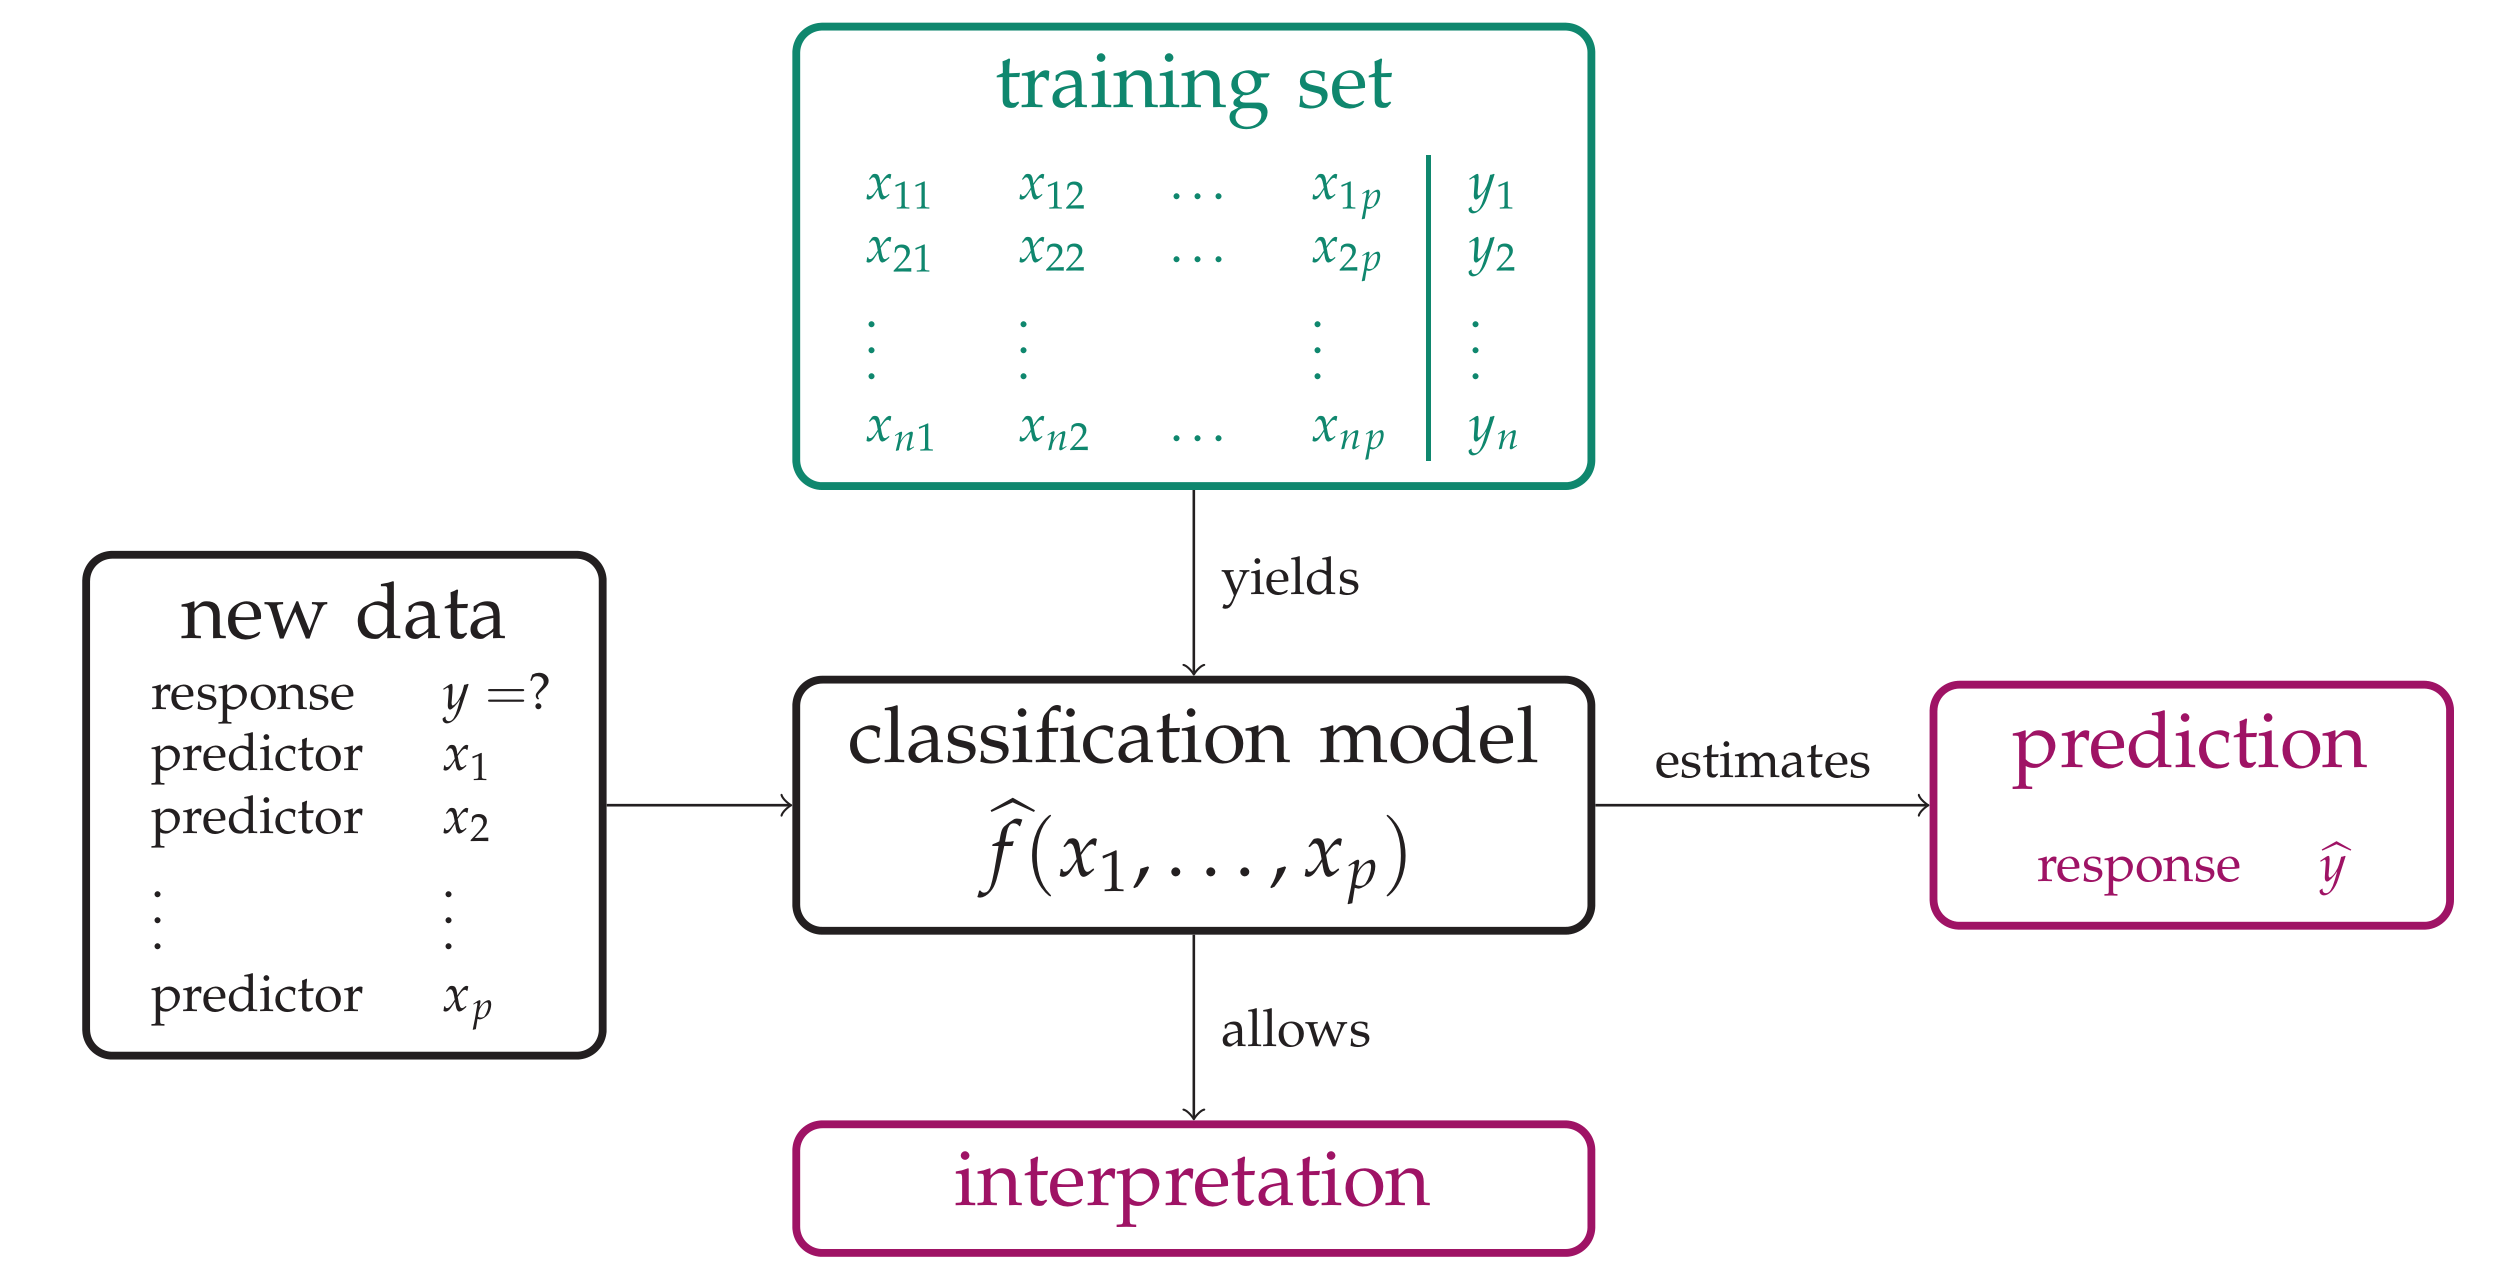
\includegraphics[width=0.6\linewidth]{img/classification}
\end{center}

Given a problem where the prediction should be whether a person defaults on their debt, based on the annual income and the monthly credit card bill, with a dataset consisting of
\begin{itemize}
	\item \predvar{default}\qquad Binary response variable, whether this person defaults or not
	\item \predvar{income}\qquad First numeric predictor, annual income of the person
	\item \predvar{balance}\qquad Second numeric predictor, monthly credit card balance
\end{itemize}

\subsection{Logistic Regression}
A model for this problem should predict the conditional probability $P(\predvar{default=Yes}|\predvar{balance})$, which is abbreviated as $p(\predvar{balance})$. Thus the aim is to model the conditional probability $p(X) = P(Y=1|X)$, where only binary response variables $Y$ are considered.

The idea underlying \emph{logistic regression} is to modify a linear function by composing it with another function which shrinks all of $\R$ to $[0,1]$. In logistic regression, the \emph{logistic} function is typically chosen
\begin{equation*}
	p(t) = \frac{e^t}{1+e^t}
\end{equation*}
\begin{center}
	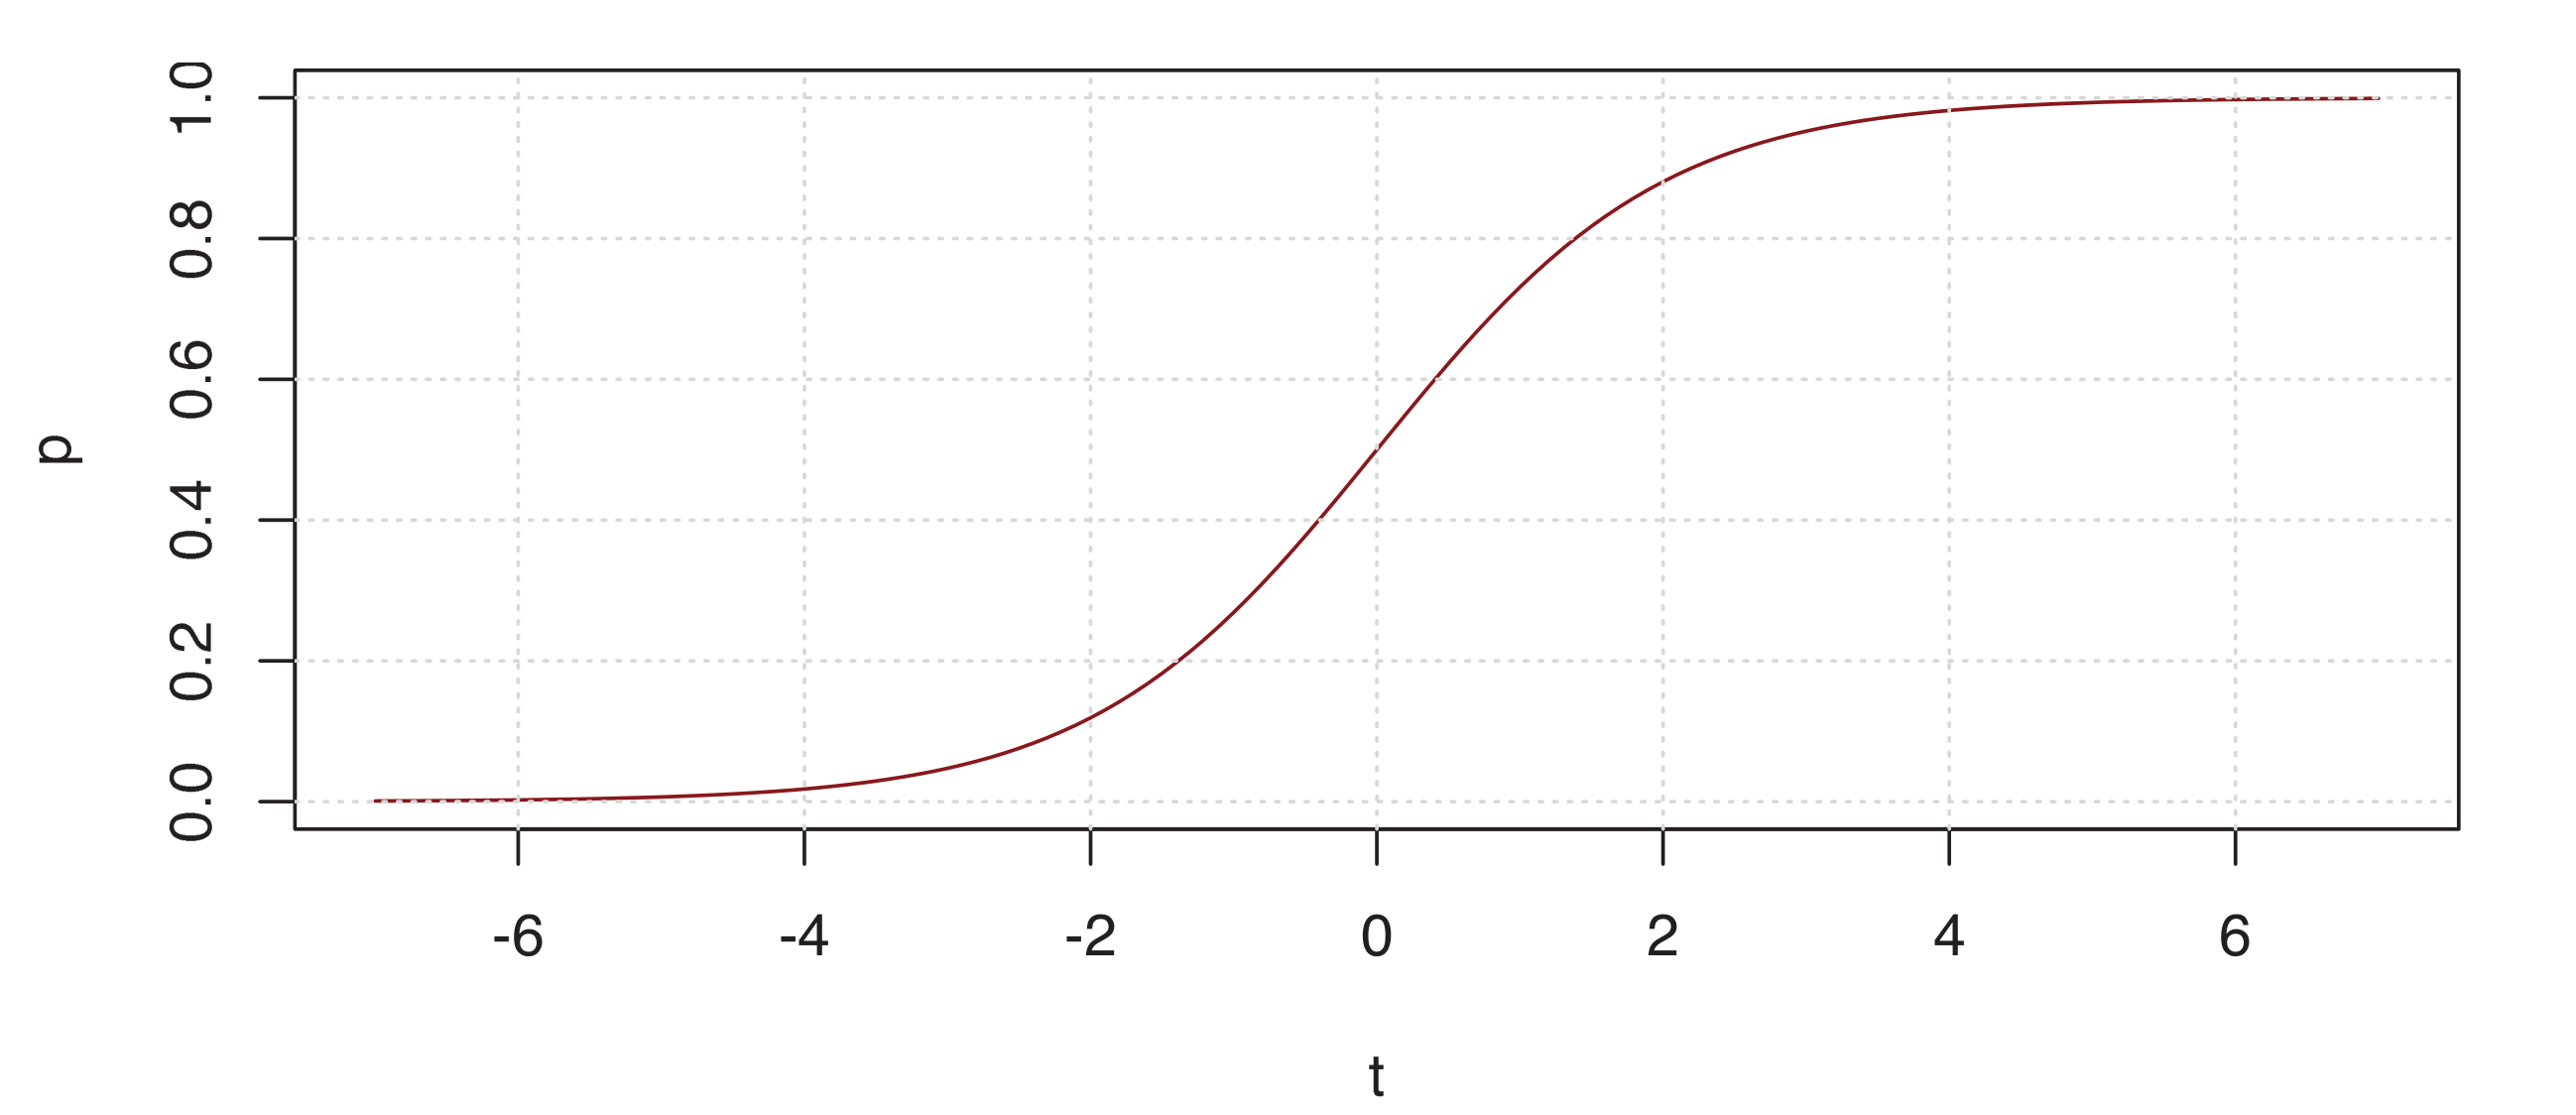
\includegraphics[width=0.4\linewidth]{img/logistic_function}
\end{center}


\begin{definition}
	\textbf{Simple logistic regression}\qquad Given a binary response variable $Y$ and a quantitative predictor $X$, the simple logistic regression model is defined as
	\begin{equation*}
		P(Y=1|X) = \frac{e^{\beta_0+\beta_1 X}}{1+e^{\beta_0+\beta_1 X}}
	\end{equation*}
	The parameters $\beta_0$ and $\beta_1$ are called regression coefficients and are estimated from the training set.
\end{definition}
Rearranging gives
\begin{equation*}
	\frac{p(X)}{1-p(X)} = e^{\beta_0+\beta_1X}
\end{equation*}
which is called \textbf{odds}. Odds is an equivalent way of expressing the probability of an event and is used for instance in betting agencies. Odds values close to 0 and $\infty$ indicate small and large probabilities, respectively.

Taking the natural logarithm of the odds gives
\begin{equation*}
	\log\left(\frac{p(X)}{1-p(X)}\right) = \beta_0+\beta_1 X
\end{equation*}
The left side of this equation is called \emph{log-odds} or \textbf{logit}. The interpretation of the coefficients $\beta_0$ and $\beta_1$ in terms of the logit: a change of the predictor $X$ by one unit amounts to an average change by $\beta_1$ of the logit of the response being true.

\subsection{Multiple Logistic Regression}
\begin{definition}
	Given a binary response variable $Y$ and predictors $X_1,\dots,X_p$, the logistic regression model is defined by
	\begin{equation*}
		P(Y|X_1,\dots,X_p) = \frac{e^{\beta_0+\beta_1 X_1 + \dots + \beta_p X_p}}{1+e^{\beta_0+\beta_1 X_1 + \dots + \beta_p X_p}}
	\end{equation*}
	The parameters $\beta_0,\beta_1,\dots,\beta_p$ are called regression coefficients and are estimated from the training set.
\end{definition}
The coefficients are estimated using the maximum likelihood function.

\subsection{Model Assessment}
\begin{definition}
	Let $(x_1, y_1),\dots,(x n_,y_n)$ be observations of $(X,Y)$ and $\hat{y}_i = \hat{f}(x_i)$ the corresponding predictions. The \emph{classification error} is given by
	\begin{equation*}
		\text{Err} = \frac{1}{n}\sum_{i=1}^{n} l(y_i \neq \hat{y}_i)
	\end{equation*}
	Where $l$ denotes the \emph{indicator function} which takes on value 1 it its argument is true and 0 otherwise. In other words, the classification error is the proportion of cases with a wrong prediction.
\end{definition}

\section{Decision Trees}
Tree-based methods can be applied for classification and regression. A classification tree aims at segmenting or stratifying the predictor space into a number of simple regions, where each region is associated with a unique class of the response. Since the set of splitting rules used to segment the predictor space can be summarized in a tree, these types of approaches are called decision-tree methods.

Tree-based methods are simple and useful for interpretation, however they are typically not competitive with supervised learning methods in terms of prediction accuracy and they overfit the training data very fast. Combining a large number of trees can often result in dramatic improvements in prediction accuracy, at the loss of some interpretation.

The idea behind a decision tree is to recursively partition the predictor variable space into disjoint regions, where each region is as pure as possible with respect to the labels of the response variable.

\begin{definition}
	Given the training set $(\vec{x}_1,y_1),\dots,(\vec{x}_n,y_n)$ where $\vec{x}_i = x_{i1}, x_{i2}, \dots, x_{ip}$ are the predictor values and $y_i$ is a qualitative response
	\begin{enumerate}
		\item Initialise the set of regions $\mathcal{R} = {R}$ by the predictor domain $R$ ($\R^p$)
		\item Choose the optimal region $R$ in $\mathcal{R}$ and the optimal predictor $X_i$ such that a \emph{binary split} of $R$ with respect to $X_i$
		\begin{equation*}
			R_1 = \left\{ \vec{x} \in \R \middle| x_i > t \right\} \quad\text{and}\quad R_1 = \left\{ \vec{x} \in \R \middle| x_i \leq t \right\}
		\end{equation*}
		gives the highest gain in purity (for some threshold $t$)
		\item Replace $R$ in $\mathcal{R}$ with $R_1$ and $R_2$ and iterate
	\end{enumerate}
	The iteration is stopped if the current splitting fulfils a pre-defined stopping criterion.
\end{definition}

\subsection{Node Purity}
Assume that the response $Y$ has $K$ levels and a tree $T$ with $M$ terminal nodes.

\vspace{1em}
\noindent
\textbf{Classification error rate}: fraction of training samples in a region that do not belong to the most common class
\begin{equation*}
	E_m(T) = 1 - \max_k \hat{p}_{mk}
\end{equation*}
$\hat{p}_{mk}$ is the proportion of the training data in region $m$ that is from level $k$. However, this classification is not sufficiently sensitive for tree growing.

\vspace{1em}
\noindent
\textbf{Gini Index}: measure of total variance across the $K$ classes 
\begin{equation*}
	G_m(T) = \sum_{k=1}^{K} \hat{p}_{mk} (1 - \hat{p}_{mk})
\end{equation*}
Gini index takes on a small value if all the $p_{mk}$ are close to zero or one. The Gini index is referred to as node purity measure. A small value indicates that a node contains predominantly observations from the same class.

\vspace{1em}
\noindent
\textbf{Cross Entropy}: an alternative to the Gini Index
\begin{equation*}
	D_m(T) = -\sum_{k=1}^{K} \log(\hat{p}_{mk})
\end{equation*}

\subsection{Making Predictions}
Once a tree has been grown from the training set, predictions for new data $\vec{x} = (x_1, \dots, x_p)$ can be made by passing $\vec{x}$ through the tree. This means applying the decision rules invoking the individual predictor values in the tree.

Assume that the decision rules lead this particular vector $\vec{x}$ to the $m$-th terminal node, that is the predictor values are within the $m$-th region $R_m$. Then the estimator $\hat{y}$ is the most commonly occurring class in the training data in region $R_m$.

\subsection{Pruning a Tree}
Growing a complex tree, that is a tree with many, small terminal nodes, will produce good predictions on the training data, but is likely to overfit the data. A smaller tree with fewer splits might lead to lower variance and better interpretation at the cost of a little bias.

One way to overcome this problem is to grow the tree only so long as the decrease in the purity measure due to each split exceeds some threshold. This will result in smaller trees, but fails to account for seemingly worthless splits early on with good splits later down in the tree.

Tree pruning amounts to first grow a very large tree and successively prune it back until a good subtree is found. Cost Complexity Pruning, also known as weakest link pruning, is used to do this.

\subsubsection{Cost Complexity Pruning}
\begin{itemize}
	\item Compute large tree $T_0$
	\item Consider a sequence of subtrees $T_\alpha$ indexed by a non-negative tuning parameter $\alpha$. For each value of $\alpha$ there is a corresponding subtree $T\subset T_0$ which minimises the cost-complexity function
	\begin{equation*}
		R_{\alpha}(T) = \sum_{m=1}^{\abs{T}} N_m Q_m (T) + \alpha\abs{T}\qquad \alpha\geq 0
	\end{equation*}
	where $\abs{T}$ denotes the number of terminal nodes in the subtree $T$, $m$ ranges over all terminal nodes, $N_m$ denotes the number of element in the terminal node $m$, and $Q_m(T)$ is an arbitrary node purity measure
	\item For each given value of $\alpha$ compute a $T_\alpha$ such that $R_{\alpha}(T)$ is minimised. $\alpha$ is a tuning parameter that controls the trade-off between complexity and fit to the training data. A large value penalises the number of terminal nodes, hence resulting in a tree with few terminal nodes, but a potentially poor fit to the training data. A small value puts all emphasis on data fit and will result in a complex tree with many terminal nodes.
\end{itemize}
\begin{enumerate}
	\item Use recursive binary splitting to grow a very large tree $T_0$ and set $\alpha = 0$
	\item Increase $\alpha$ and compute the subtree $T_\alpha$ that minimises the cost-complexity function $R_\alpha(T)$ for each value
	\item Stop if $T_\alpha$ is the root node
\end{enumerate}
To compute $T_\alpha$ weakest link cutting is used, which amounts to successively collapse the internal node that leads to the smallest increase in $R(T)$ until the tree with a single node is reached. The sequence of trees generated by this procedure can be shown to contain $T_\alpha$.

\subsubsection{Optimal Pruning by Cross-Validation}
Divide the data set into $K$ folds. For $k = 1,\dots,K$
\begin{enumerate}
	\item Grow a large tree $T_0$ based on all but the $k$-th fold of the data set.
	\item Perform cost-complexity pruning and obtain a sequence of optimal subtrees $T_\alpha$ as a function of $\alpha$. Compute the classification error rate on the $k$-th fold as a function of $\alpha$.
\end{enumerate}
For each value of $\alpha$ average the classification error rate over the $K$ folds. Choose $\alpha$ such that the error rate is minimal.

\section{Bagging and Random Forests}
\subsection{Review Decision Trees}
\textbf{Advantages}
\begin{itemize}
	\item Comprehensible and versatile with respect to the predictors
	\item Can be visualised nicely and in a comprehensive manner
\end{itemize}

\vspace{1em}
\noindent
\textbf{Disadvantages}
\begin{itemize}
	\item Poor predictive accuracy, especially when generalising
	\item High variance\\
	Splitting the training data into two parts at random and fitting a tree on both results in quite different trees
\end{itemize}

\subsection{Bagging}
Bagging is a statistical tool that allows reducing the variance of a statistical estimator. It is based on the aggregation of a multitude of estimators with high variance by means of averaging and thus reducing the variance. These estimators are created by bootstrapping the training data (\textbf{b}ootstrap \textbf{agg}regat\textbf{ing}). Random Forests are a further advancement of bagging being a relevant classification method for real world problems.

\subsection{Bootstrapping}
Each of these bootstrap data sets is created by sampling with replacement and is the same size as the original data set. As a result, some observations may appear more than once in a given bootstrap data set and some not at all. Thus, rather than repeatedly obtaining independent data sets from the population, distinct data sets are obtained by sampling the observations from the original data set.

\newpage
\begin{definition}
	Let $x_1,\dots, x_n$ be, possibly multivariate, realisations of the independent and identically distributed random variables $X_1, \dots, X_n$. Assume further that
	\begin{equation*}
		\hat{\gamma} = \hat{\gamma}(x_1, \dots, x_n)
	\end{equation*}
	is an estimator of some quantity $\gamma$.
	\begin{enumerate}
		\item Choose a large number $B\in \mathbb{N}$
		\item For $b = 1,\dots,B$
		\begin{itemize}
			\item Draw $n$ samples $\left\{ x_1^{*}, \dots, x_n^{*} \right\}$ from $\left\{ x_1, \dots, x_n \right\}$ with replacement
			\item Compute the estimator $\hat{\gamma}^{*} = \hat{\gamma}(x_1^{*}, \dots, x_n^{*})$
		\end{itemize}
	\end{enumerate}
	\item The empirical distribution function $\hat{F}^*$ of $ \left( \hat{\gamma}_1^{*},\dots,\hat{\gamma}_n^{*} \right)$ approximates the distribution of $\hat{\gamma}$. In particular, the standard error of $\hat{\gamma}$ can be estimated by the bootstrap estimate
	\begin{equation*}
		\text{se}_B(\hat{\gamma}) = \sqrt{\frac{1}{B-1}\sum_{b=1}^{B}(\hat{\gamma}_n^{*} - \samplemean{\gamma}^{*})^2},\qquad\text{with } \samplemean{\gamma}^{*} = \frac{1}{B}\sum_{b=1}^{B}\hat{\gamma}_b^*
	\end{equation*}
\end{definition}

Bagging is a general-purpose procedure for reducing the variance of a statistical learning method. It is particularly useful and frequent in the context of decision trees. By averaging the variance is reduced. A more natural way to decrease the variance of a statistical learning method and hence to increase the predictive accuracy would be to take many training sets from the population, build a separate prediction model using each training set, and average the resulting predictions. This is not practical, as only one training set can be accessed most of the time.

For a regression setting (each of the $\hat{f}_b^*$ is a linear regression model) the bagged model is simply the average
\begin{equation*}
	\hat{f}_{\text{bag}}(x) = \frac{1}{B} \sum_{i=1}^{B} \hat{f}_i^*(x)
\end{equation*}

For classification, the predicted classes of all $B$ models are recorded, and the most commonly occurring class among the $B$ predictions is used. This method is called the \textbf{majority vote}.

There is a very straightforward way to estimate the test error of a bagged model, without the need to perform cross-validation or the validation set approach. It can be shown, that on average each bagged tree makes use of around \textbf{two-thirds} of the observation. The remaining \textbf{one-third} of the observations not used to fit a given bagged tree is referred to as the \textbf{out-of-bag (OOB)} observations. The response for the $i$th observation can be predicted using each of the trees in which that observation was OOB.

\newpage
\subsubsection{Out-of-bag Error Estimate}
\begin{definition}
	Let $(\vec{x}_1,y_1),\dots,(\vec{x}_n,y_n)$ be the training set and $\hat{f}_1^*,\dots,\hat{f}_b^*$ be $B$ bootstrapped classification methods, that is decision trees
	\begin{enumerate}
		\item For $i=1,\dots,n$ find all bootstrapped models $\hat{f}_b^*$ that do \textbf{not} use the $i$th observation for training. Use these models to make a prediction $\hat{y}_i^*$ by means of a majority vote.
		\item The out-of-bag error estimate is the classification error
		\begin{equation*}
			\text{Err}^* = \frac{1}{n}\sum_{i=1}^{n}l(y_i\neq \hat{y}_i^*)
		\end{equation*}
	\end{enumerate}
\end{definition}
The resulting OOB error is a valid estimate of the test error for the bagged model, since the response for each observation is predicted using only the trees that were not fit using that observation. It can be shown that with $B$ sufficiently large (usually $B=1000$ samples are sufficient), OOB error is virtually equivalent to leave-one-out cross-validation error.

\subsection{Random Forests}
Random forests provide an improvement over bagged trees by way of a small tweak that \textbf{decorrelates} the trees. As with bagging, a number of decision trees are fitted on bootstrapped training samples. But when building these decision trees, each time a split in the tree is considered, a \textbf{random sample of $\bm{m}$ predictors} is chosen as split candidates from the full set of $p$ predictors. A split in the decision tree is allowed to use \textbf{only one of those $\bm{m}$ predictors}.

A fresh sample of $m$ predictors is taken at each split, and $m\approx \sqrt{p}$ is chosen. Thus, the number of predictors considered at each split is approximately equal to the square root of the total number of predictors. The rationale behind this is: Suppose that there is one very strong predictor in the data set, along with a number of other moderately strong predictors. Most or all of the trees in the collection of bagged trees will use this strong predictor in the top split. 

Consequently, all of the bagged trees will look quite similar to each other and the predictions from the bagged trees will be highly correlated. Unfortunately, \textbf{averaging many highly correlated quantities} does \textbf{not} lead to as large of a reduction in variance as averaging many uncorrelated quantities.

Bagging typically results in improved accuracy over prediction using a single tree. Unfortunately, it can be difficult to interpret the resulting model. Thus, bagging improves the accuracy \textbf{at the expense of interpretability}. One can obtain an overall summary of the importance of each predictor using the Gini index, by adding up the total amount that the Gini index is decreased by splits over a given predictor, averaged over all $B$ trees.

\section{Time Series Analysis}

\begin{figure}[H]
	\centering
	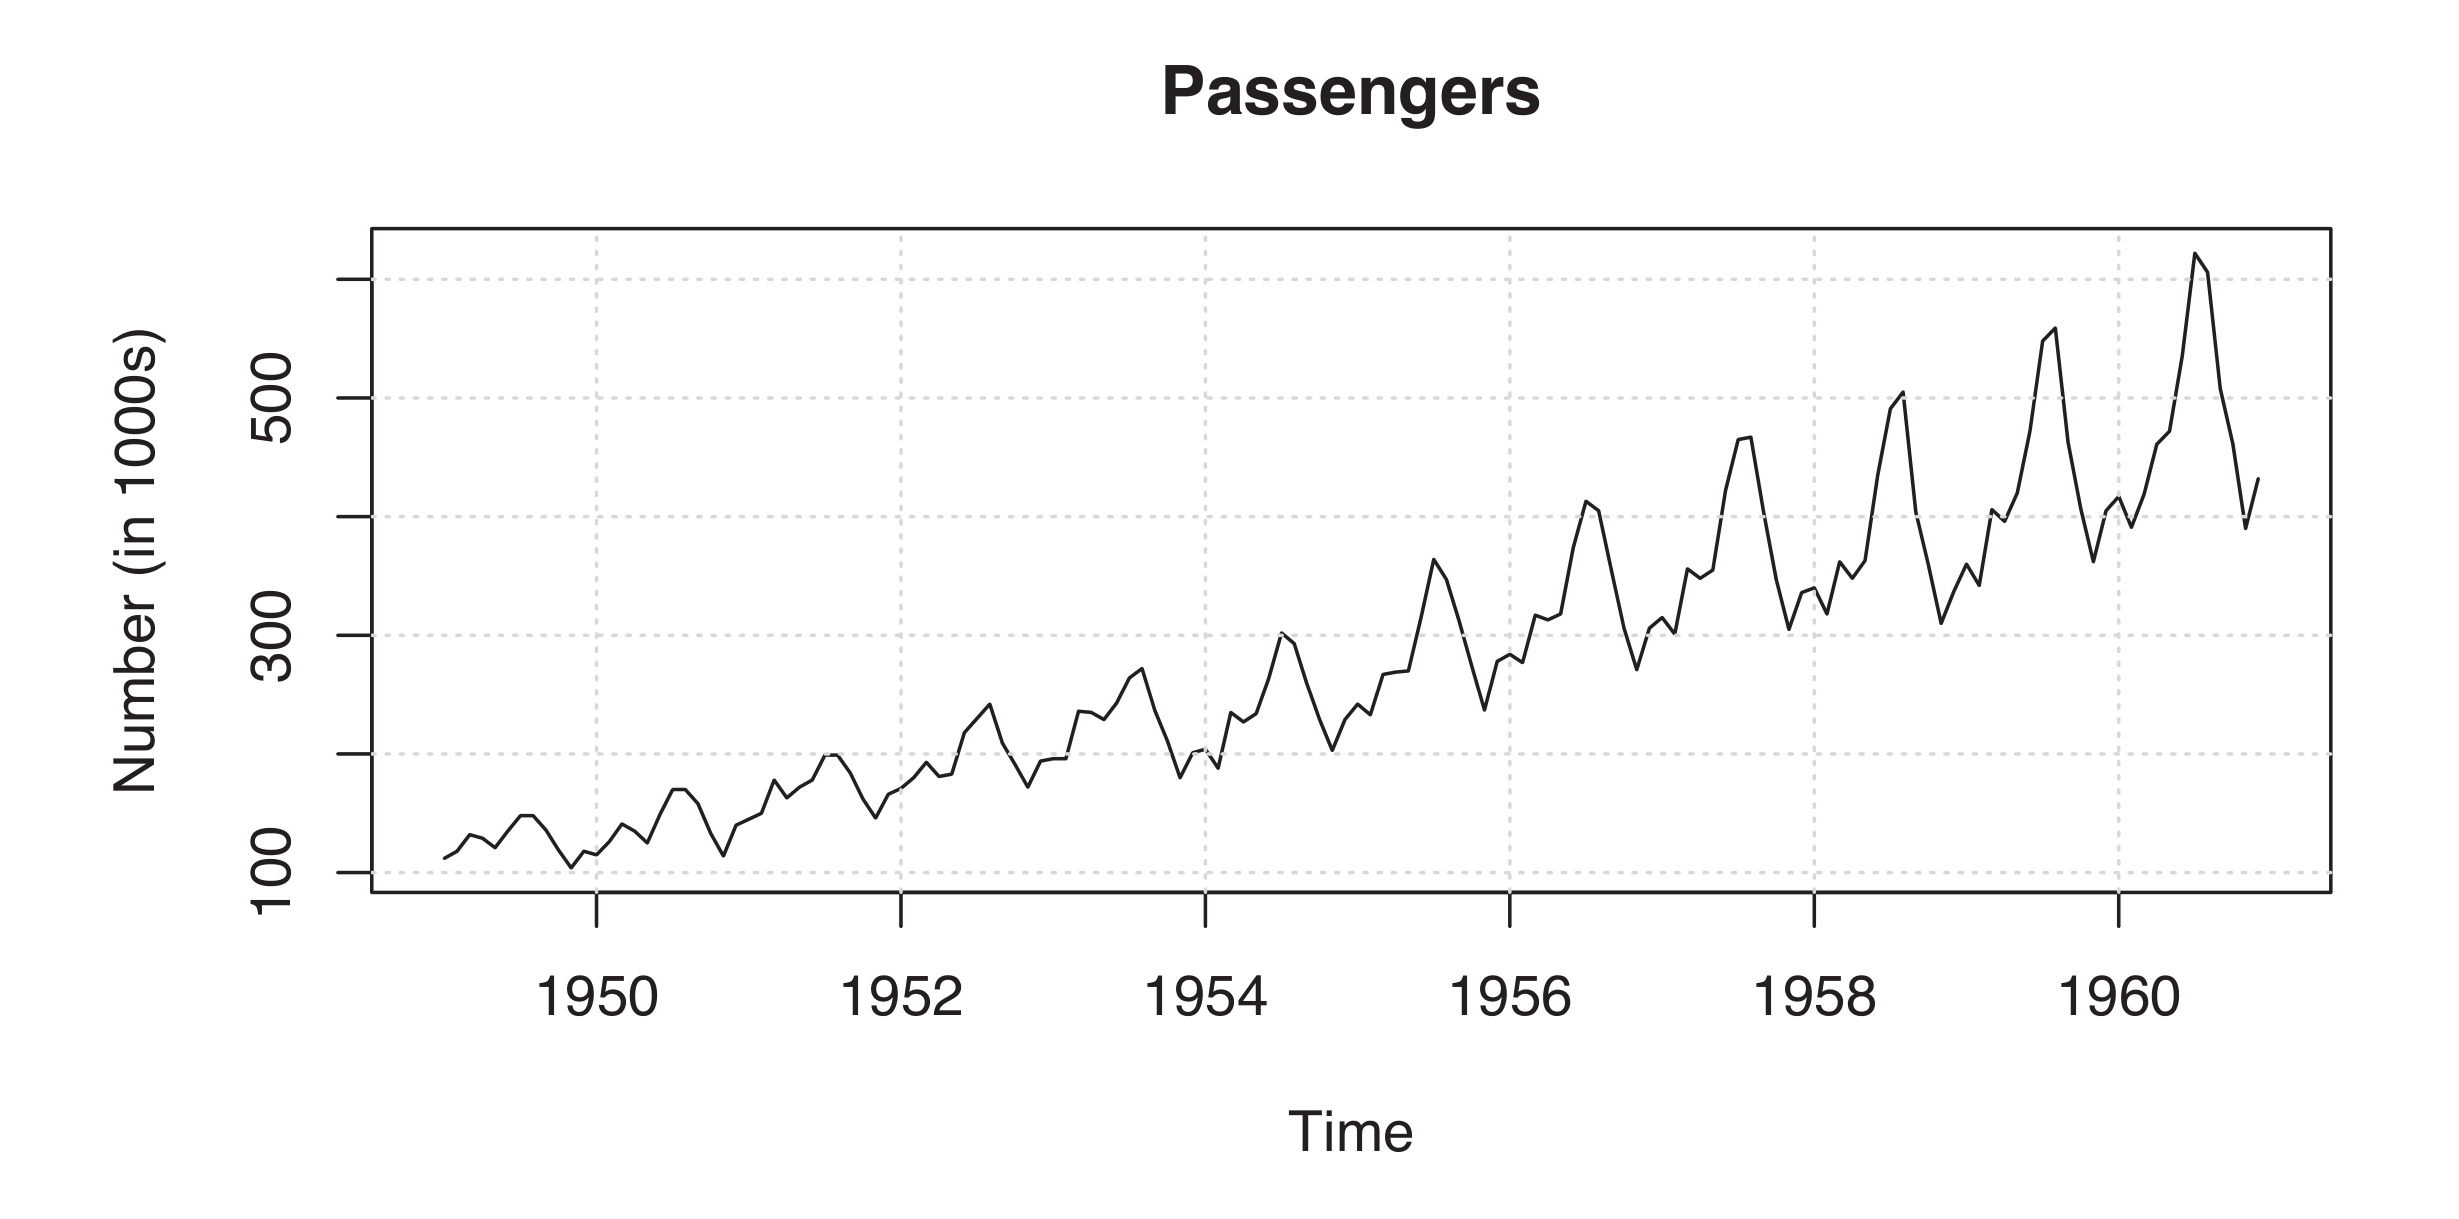
\includegraphics[width=0.7\linewidth]{img/time_series_plot}
	\caption{Number of airline passenger bookings (in thousands) per month of the airline PanAm from 1949 to 1960}
	\label{fig:timeseriesplot}
\end{figure}
The following patterns become visible, the global increase of flight bookings over time (\textbf{trend}), there are more flight bookings during summer months (\textbf{seasonality}) and that the observations are \emph{not} independent (\textbf{serial correlation}).

Many real life measuring and data recording processes result in data sets that are serially correlated. Examples are machine monitors (temperature, pressure, acoustic emissions, vibrations, any signals measured in, at or around an operating engine), stocks (stock prices and exchange rates are recorded at the end of each day), environmental observations (temperature, humidity, pollen concentration, pollution, precipitation and other signals recorded at a specific station), and federal statistics. This kind of data is called \emph{time series data}. 

With time series analysis the following goals can be achieved
\begin{enumerate}
	\item \textbf{Descriptive Analysis}\\
	Understand the basic properties of a time series by means of summary statistics and visualisations.
	\item \textbf{Modelling and Interpretation}\\
	Gain a deeper understanding by modelling the underlying process that governs the observed time series. In particular, tests and confidence intervalls/bands can be constructed from the model. The sequential dependency of the time series is also often quantified.
	\item \textbf{Decomposition}
	\begin{itemize}
		\item \emph{Seasonality}, in particular a periodic pattern in the data
		\item \emph{Trend}, gradually changing average of the series which is directly correlated with the time axis
	\end{itemize}
	\item \textbf{Prediction}\\
	Predict future values of the time series by using the model. Prediction for time series is often alternatively termed \emph{forecasting}.
	\item \textbf{Regression}\\
	Try to explain a time series or \emph{response} by several other time series called \emph{predictors}. This idea is wide-spread in the industry, where the goal is to replace in a multi-sensor setup a particular sensor by a model that predicts its values from the other sensor values. This is called \emph{virtual sensoring} or \emph{soft sensoring}.
\end{enumerate}

\subsection{Basic Transformation, Visualisation and Decomposition of Time Series}
Analysis of time series begins with the description, transformation and visualization of data. This does not give proper predictions or confidence intervals. Important insights and a profound understanding of the data can be achieved by these techniques. It is often desirable or even necessary to transform a time series before the application of models and predictions. In particular, many methods assume a
\begin{itemize}[nosep]
	\item \textbf{Gaussian} or at least \textbf{symmetric} distribution of the data
	\item \textbf{Linear} trend relationship between time and data
	\item \textbf{Constant variance} across time
\end{itemize}
For a highly skewed or heteroscedastic data it is often better to use a transformed series $\left\{g(x_1), g(x_2), \dots\right\}$ in stead of the original series $\left\{x_1,x_2,\dots\right\}$. A family of transformations, that is well suited for correcting skewness and variance are the Box-Cox-transformations.
\begin{definition}
	For a time series $\left\{x_1,x_2,\dots\right\}$ with positive values the \textbf{Box-Cox transformations} are defined as
	\begin{equation*}
		g(x) = \left\{\begin{matrix}
		\frac{x^\lambda - 1}{\lambda} & \text{if } \lambda \neq 0\\
		\log(x) & \text{if } \lambda = 0
		\end{matrix}\right.
	\end{equation*}
\end{definition}
The Box-Cox family of transforms amounts to a modification of the values of the time series. Sometimes it is necessary to transform the time-axis as well. The most simple version of time transforms is \emph{shifting}
\begin{definition}
	Let $\left\{x_1,x_2,\dots\right\}$ be a time series
	\begin{enumerate}
		\item The time-shift ba a \emph{lag} of $k\in\Z$ is defined by
		\begin{equation*}
			g(x_i) = x_{i-k}
		\end{equation*}
		\item For the particular case where $k=1$ the time-shift is called \emph{backshift}
		\begin{equation*}
			B(x_i) = x_{i-1}
		\end{equation*}
	\end{enumerate}
\end{definition}
Applying a time-shift to a time series amounts to go back $k$ steps (if $k > 0$) or go ahead $-k$ steps (if $k < 0$) in the series

\subsubsection{Log-Returns}
Back-shift operator is applied when \emph{differences} of time series are computed, since
\begin{equation*}
	x_i - x_{i-1} = x_i - B(x_i)
\end{equation*}
Differencing is often combined with Box-Cox transformations. The \textbf{log-returns} of a (financial) time series are defined as
\begin{equation*}
	y_i = \log(x_i) - \log (x_{i-1}) = log\left(\frac{x_i}{x_{i-1}}\right) = \log\left(\frac{x_i - x_{i-1}}{x_{i-1}} + 1\right) \approx \frac{x_i - x_{i-1}}{x_{i-1}}
\end{equation*}
The log-returns of time series $y_i$ approximates the relative increase of the time series $x_i$ at each time instance. This quantity is often studied in financial applications, as the original series may exhibit \emph{seemingly significant patterns}, but the resulting series $y$ is often rather \emph{random}. The log-return looks quite random despite some large fluctuations from time to time. Analysts try to model the waiting time between these fluctuations.

\subsubsection{Decomposition}
Many time series are dominated by a trend or seasonal effects, or both. A simple \textbf{additive} decomposition model is given by
\begin{equation*}
	x_k = m_k + s_k + z_k
\end{equation*}
where $k$ time index, $x_k$ observed time series, $m_k$ trend, $s_k$ seasonal effect, and $z_k$ error term that is, in general, a sequence of correlated random variables with mean zero.

In the air passengers data the seasonal effects may increase as the trend increases. Thus, a \textbf{multiplicative} model seems more appropriate
\begin{equation*}
	x_k = m_k \cdot s_k + z_k
\end{equation*}
If the noise is multiplicative as well ($x_k = m_k \cdot s_k \cdot z_k$) the logarithm of $x_k$ is a linear model again
\begin{equation*}
	\log(x_k) = \log(m_k) + \log(s_k) + \log(z_k)
\end{equation*}

\subsubsection{Moving Average}
The moving average is a method for estimating the \textbf{trend} $m_k$ and the \textbf{seasonal effect} $s_k$ by means of a moving average filter.
\begin{definition}
	Assume that $\left\{x_1,x_2,\dots, x_n\right\}$ is a time series and that $p\in\mathbb{N}$. The \emph{moving average filter} of length $p$ is defined as follows
	\begin{itemize}
		\item If $p$ is odd, the $p = 2l + 1$ and the filtered sequence is defined by
		\begin{equation*}
			g(x_i) = \frac{1}{p} (x_{i-l} + \dots + x_i + \dots + x_{i+l})
		\end{equation*}
		\item If $p$ is even, then $p = 2l$ and the filtered sequence is defined by
		\begin{equation*}
			g(x_i) = \frac{1}{p} (\frac{1}{2}x_{i-l} + x_{i-l+1} + \dots + x_i + \dots + x_{i+l-1} + \frac{1}{2} x_{i+l})
		\end{equation*}
	\end{itemize}
	The value $p$ is referred to as window width.
\end{definition}
The moving average filter amounts to replace the $i$-th value in the time series by the average of the $p$ nearest neighbours of $x_i$. If $p$ is odd, then the window stretches symmetrically around $x_i$. For an even $p$ the window length is $p+1$ but the end points are only counted half.

If a time series has the frequency $p$ ($p = 12 $for monthly data), then the trend component of the time series can be estimated by applying the moving average filter with window width $p$. Since the average at each point is exactly over one period, the seasonal effects vanish and the trend component remains. This yields the trend estimator $\hat{m}_k$. To estimate the seasonal additive effects compute
\begin{equation*}
	\hat{s}_k = x_k - \hat{m}_k
\end{equation*}
With this the time series $\hat{s}_k$ is averaged for each time point in one cycle, and a single estimate can by obtained for each cycle point. The residuals can be obtained by subtracting the trend and seasonality estimates
\begin{equation*}
	\hat{r}_i = x_i - \hat{m}_i - \hat{s}_i
\end{equation*}
The remainder term should consists of possibly correlated random values without structure or periodicity.

\subsection{Seasonal Decomposition by LOESS}
Although the decomposition method gives promising results for the example data sets, it is rarely used in practice as it lacks robustness with respect to outliers in the data, and the seasonal component is assumed to be constant over time. The state of the art method for decomposing time series that does not suffer from the above drawbacks is \emph{seasonal decomposition of time series by LOESS} (STL). The STL procedure is iterative, outliers in the estimated remainder terms are detected and their effect mitigated by proper reweighing.

The moving average smoothing is replaced by \emph{locally estimated scatterplot smoothing} (LOESS) regression which gives more flexibility and better results than the moving average. LOESS regression is a form of \emph{local} regression which means that the regression line through data $(x_1, y_1 ),\dots,(x_n, y_n)$ at a point $x$ is only computed using the observations in a neighbourhood of $x$.

The seasonal  component is not assumed to be constant. The method instead considers \emph{cycle-subseries}, that is the subseries of values at each position of the seasonal cycle. For example, for a monthly series with frequency $12$, the first cycle-subseries consists of the January values, the second of the February values. These sub-cycles are also smoothed by LOESS and may change over time.

\section{Mathematical Models for Time Series}
For describing characteristics of data that seemingly fluctuate in a random fashion over time, a time series can be considered as the realization of random variables that are indexed over time.

\begin{definition}
	\textbf{Time Series and Discrete Stochastic Processes}: Let $T$ be a set of equidistant time points $T =\{t_1, t_2, \dots\}$.
	\begin{enumerate}
		\item A \emph{discrete stochastic process} is a set of random variables $\{X_1, X_2, \dots\}$. Each single random variable $X_i$ has a univariate distribution function $F_i$ and can be observed at time $t_i$.
		\item A \emph{time series} $\{x_1, x_2, \dots\}$ is a realisation of a discrete stochastic process $\{X_1,X_2,\dots\}$. In other words, the value $x_i$ is a realisation of the random variable $X_i$ measured at time $t_i$
	\end{enumerate}
\end{definition}
Important distinction between a time series, which are a concrete observation of values, and a discrete stochastic process which is a theoretical construct to model the underlying mechanism that generates the values.

A time series $\{x_1, x_2, \dots, x_N\}$ can be understood as \emph{one} realisation of a multivariate random variable $\{X_1, X_2, \dots, X_N\}$. Modelling and prediction for time series hence amounts to analyse a data set with one observation, which is impossible without further assumptions on the series. A model that lacks all these assumptions and thus is unpredictable is \textbf{white noise}.

\subsection{Moving Average from White Noise Process}
\begin{itemize}
	\item Apply a sliding window filter to obtain a \textbf{moving average} process
	\begin{equation*}
		\{ W_1, W_2, \dots\}
	\end{equation*}
	\item Choose a window length $w$
	\begin{equation*}
		V_i = \frac{1}{w} \left( W_{i-\frac{w}{2}} + \cdots + W_i + \cdots + W_{i+\frac{w}{2}} \right)
	\end{equation*}
	\item The resulting process is smoother through smoothing out the higher oscillations
\end{itemize}

\subsection{Autoregressive Time Series}
Many examples of real world time series, for example acoustic time series in speech analysis, contain dominant oscillatory components, producing a sinusoidal type of behaviour. One possible model to generate such quasi-periodic data are \textbf{autoregressive series}.
\begin{equation*}
	X_i = \alpha_1 X_{i-1} + \alpha_2 X_{i-2} + W_i
\end{equation*}
In other words, the value of the process at time instance $i$ is modelled as a linear combination of the past two values plus some random component. Therefore this process is called autoregressive.

Another interpretation of the autoregressive process above is via differential equations. The finite difference scheme for the second order equation
\begin{align*}
	\ddot{x} + 2\theta \dot{x} + \omega_0^2 x = W(t)
	\intertext{is given by}
	\frac{x_{i-2} - 2x_{i-1} + x_i}{\Delta t^2} + 2\theta\frac{x_{i-1}-x_i}{\Delta t} + \omega_0^2 = W_i
\end{align*}
Here $\theta$ is the damping term and $\omega_0$ the frequency of the homogeneous equation. Hence it can be seen as a \textbf{harmonic oscillator with random input}.

\subsection{Measures of Dependence}
Aside from the individual distributions $F_i$ of the random variables in the process, we define \textbf{first} and \textbf{second order} moments to analyse the whole process.
\begin{definition}
	The \textbf{mean sequence} $\{\mu(1),\mu(2), \dots\}$ of a discrete stochastic process\\
	$\{X_1, X_2, \dots\}$ is defined as the sequence of the means
	\begin{equation*}
		\mu(i) = \ev{X_i}
	\end{equation*}
\end{definition}

\noindent
\textbf{Autocovariance} and \textbf{Autocorrelation}
\begin{definition}
	Let $\{X_1, X_2, \dots\}$ be a discrete stochastic process
	\begin{enumerate}
		\item The \emph{autocovariance} $\gamma_X$ is defined as
		\begin{equation*}
			\gamma_X(i,j) = \Cov{X_i,X_j} = \ev{(X_i - \mu(i))(X_j - \mu(j))}
		\end{equation*}
		\item The \emph{autocorrelation} $\rho_X$ is defined as
		\begin{equation*}
			\rho_X(i,j) = \frac{\gamma_X(i,j)}{\sqrt{\gamma_X(i,i)\gamma_X(j,j)}}
		\end{equation*}
	\end{enumerate}
\end{definition}
The autocovariance measures the linear dependence of two points on the same process observed at different times. If a series is very smooth, the autocovariance is large, even if $i$ and $j$ are far apart.

\clearpage
\subsection{Stationarity}
\begin{definition}
	A discrete stochastic process is called \emph{strictly stationary} if for each finite collection $\{X_{i_1}, \dots, X_{i_n}\}$ and each lag $h\in\Z$ the shifted collection
	\begin{equation*}
		\{X_{i_1+h}, \dots, X_{i_n+h}\}
	\end{equation*}
	has the same distribution. Put differently
	\begin{equation*}
		P(X_{i_1}\leq c_1, \dots, X_{i_n}\leq c_n) = P(X_{i_1+h}\leq c_1, \dots, X_{i_n+h}\leq c_n)
	\end{equation*}
	for any $c_1,\dots,c_n$
\end{definition}
In words, the probabilistic character of the process does not change over time. This amounts to say that the marginal distributions $F_i = F$ of the process coincide and in particular this implies that the \textbf{mean sequence is constant}.

\begin{definition}
	A discrete stochastic process $X_i$ is called \emph{weakly stationary} if
	\begin{enumerate}
		\item the mean sequence $\mu_X(i)$ is constant and does not depend on the time index $i$
		\item the autocovariance sequence $\gamma_X(i,j)$ depends on $i$ and $j$ only through their difference $\abs{i-j}$
	\end{enumerate}
\end{definition}

If a process is stationary the mean sequence is constant, thus a canonical estimator is
\begin{equation*}
	\hat{\mu} = \samplemean{x} = \frac{1}{n}\sum_{i=1}^n x_i
\end{equation*}
\begin{definition}
	\textbf{Sample Autocovariance}
	\begin{enumerate}
		\item The \emph{sample autocovariance} is defined by
		\begin{equation*}
			\hat{\gamma}(h) = \frac{1}{n}\sum_{i=1}^{n-h}(x_{i+h}-\samplemean{x})(x_i - \samplemean{x})
		\end{equation*}
		with $\hat{\gamma}(-h) =\hat{\gamma}(h)$ for $h=0,1,\dots,n-1$
		\item The \emph{sample autocorrelation} is defined by
		\begin{equation*}
			\hat{\rho}(h) = \frac{\hat{\gamma}(h)}{\hat{\gamma}(0)}
		\end{equation*}
	\end{enumerate}
\end{definition}

\section{Forecasting}

The goal of forecasting is to model a given time series data with a proper stochastic process to forecast future, unobserved values of the process. In other words, predict future values $x_{n+k}$ with $k=1,2,\dots$ given a time series up to the present time $\{x_1,\dots,x_n\}$.

\subsection{Procedure}
\begin{enumerate}
	\item Ascertain that the underlying process is \textbf{predictable}, that is the process will not change dramatically in the future and will continue as it has to the present
	\item Choose a \textbf{model class} by explorative data analysis of the given time series. After that, \textbf{fit} the model to the training data and receive model parameters that fully describe the fitted model
	\item \textbf{Predict} the future values of the process with the fitted model
\end{enumerate}

\subsection{Autoregressive Models}
Autoregressive models are based on the idea that the current value of the series can be explained by a linear combination of $p$ previous values
\begin{definition}
	The autoregressive model $AR(p)$ of order $p$ is a discrete stochastic process that satisfies
	\begin{equation*}
		X_n = a_1 X_{n-1} + a_2 X_{n-2} + \dots + a_p X_{n-p} + W_n
	\end{equation*}
	where $a_1,a_2,\dots,a_p$ are the model parameters and $W_1, W_2, \dots$ is a white noise process with variance $\sigma^2$. For a given autoregressive process, the \textbf{characteristic polynomial} is defined as
	\begin{equation*}
		\Phi(x) = 1 - a_1 x - a_2 x^2 - \dots - a_p x^p
	\end{equation*}
\end{definition}

Autoregressive models are \textbf{exclusively} used for the modelling of \textbf{stationary} processes. There is a sufficient  condition on the parameters of an autoregressive process that render the process stationary.
\begin{definition}
	\textbf{Stationarity of $AR(p)$}
	An $AR(p)$ stochastic process is weakly stationary, if all (complex) roots of the characteristic polynomial
	\begin{equation*}
		\Phi(x) = 1 - a_1 x - a_2 x^2 - \dots - a_p x^p
	\end{equation*}
	exceed 1 in absolute value.
\end{definition}
If the intent is to \textbf{fit an autoregressive model} to a given time series data set, two things have to be clarified in advance
\begin{enumerate}
	\item Is the \textbf{autoregressive model} the right choice for the given data
	\item What is the proper \textbf{model order} $p$ for the given data
\end{enumerate}
In practice a sample autocorrelation of a given series is computed and compared with the theoretical autocorrelation of the $AR(p)$ model. This way, it can be determined if the time series is autoregressive. Partial autocorrelation is introduced as a further measure well suited for determining the order of an autoregressive model.

The autocorrelation of an $AR(p)$ process is non-zero for a wide span of lags. This is due to propagation of correlation through the model: If $X_k$ is strongly correlated with $X_{k+1}$ and this in turn is strongly correlated with $X_{k+2}$, then $X_k$ will likely be correlated with $X_{k+2}$ as well. If the goal is to study the \textbf{direct} correlation between $X_k$ and $X_{k+2}$, that is the proportion of correlation that is \textbf{not} due to $X_{k+1}$, the \textbf{partial autocorrelation} has to be computed.

\begin{definition}
	For a weakly stationary stochastic process $\{X_1,X_2,\dots\}$ the partial autocorrelation is defined as
	\begin{equation*}
		\pi(h) = \Cor{X_k,X_{k+h}\middle|X_{k+1},\dots,X_{k+h-1}}
	\end{equation*}
	The quantity $\Cor{X,Y|Z}$ denotes the conditional correlation of $X$ and $Y$ given the value of $Z$
\end{definition}
Important properties of the partial autocorrelation
\begin{enumerate}
	\item The $p$-th coefficient $\alpha_p$ of an $AR(p)$ process equals $\pi(p)$, that is the partial autocorrelation value at lag $p$ of the process
	\item For an autoregressive process $AR(p)$ the partial autocorrelation at lags greater than $p$ is zero, that is $\pi(k) = 0$ for $k>p$
\end{enumerate}

\subsection{Model Fitting Procedure}
The estimation of an $AR(p)$ model from given time series data under the assumption that the time series is a realisation of a stationary stochastic process can be obtained by the following fitting procedure
\begin{enumerate}
	\item Decide whether a given time series stems from an autoregressive process, by investigating the autocorrelation and partial autocorrelation of the sequence. If the autocorrelation is decaying exponentially to zero (possibly with oscillations) and the partial autocorrelation is zero for larger lags, then the autoregressive model is appropriate
	\item Choose the \textbf{largest lag} $p$ such that the partial autocorrelation is \textbf{not} zero
	\item Choose parameters $a_1,\dots,a_p$ such that given data are likely to be realisations of corresponding autoregressive process
\end{enumerate}
Given the data $\{x_1,x_2,\dots,x_n\}$ and a model order $p$, an $AR(p)$ process can be fitted by solving the following linear equation system
\begin{align*}
	x_{p+1} &= a_1 x_p + a_2 x_{p-1} + \dots + a_p x_1 + W_{p+1}\\
	x_{p+2} &= a_1 x_{p+1} + a_2 x_{p} + \dots + a_p x_2 + W_{p+2}\\
	&\vdots \\
	x_n &= a_1 x_{n-1} + a_2 x_{n-2} + \dots + a_p x_{n-p} + W_{p+1}
\end{align*}
This system can be solved with
\begin{itemize}
	\item Least Squares Method
	\item Burg's algorithm
	\item Yule-Walker
	\item Maximum Likelihood Method
\end{itemize}

\subsection{Forecasting $AR(p)$ Processes}
The general methodology of forecasting stationary time series can be summarized as follows
\begin{definition}
	\textbf{$k$-step ahead forecast}
	Assume that $\{X_1,X_2,\dots\}$ is a stationary process and that there is a observation of a time series $\{x_1,x_2,\dots,x_n\}$. The $k$-steps ahead forecast is an estimate of the random variable $X_{n+k}$ given by
	\begin{equation*}
		\hat{X}_{n+k} = \ev{X_{n+k}\middle| X_1=x_1,\dots, X_n = x_n}
	\end{equation*}
	Here $\ev{X|Y=y}$ denotes the  conditional expectation of $X$ given $Y = y$
\end{definition}
A k-step ahead forecast of an $AR(1)$ process is exponentially decaying to zero from the last observation $x_n$ and does not dependent on earlier observations.

The standard error $\sigma_k$ of an autoregressive process is the square root of the conditional variance
\begin{equation*}
	\sigma_k^2 = \Var{X_{n+k}|X_1= x_1,\dots, X_n = x_n}
\end{equation*}
This quantity is increasing with $k$ and converges to the process variance $\sigma_K^2$

\clearpage
\appendix

\section{R-Code}
\subsection{Introduction to R}
\begin{minted}{R}
data <- read.table(file="./child.txt", header=TRUE, sep=",")
dim(data)
> 30 21
summary(data)
# row with lowest 'infant mortality'
index_lowest_infant_mortality <- which.min(data[,"Infant.mortality"])
index_lowest_infant_mortality
> 12
mean(data[,"Physical.activity"], na.rm=T)
\end{minted}

\subsection{QQPlot}
\begin{minted}{R}
options(repr.plot.width=20, repr.plot.height=7)
dfs = c(20,7,3)
par(mfrow = c(1,3))

for (df in dfs){
	x <- rt(20, df=df)
	qqnorm(x)
}

par(mfrow = c(1,3))
for (df in dfs){
	x <- rt(100, df=df)
	qqnorm(x)
}
\end{minted}
















\end{document}
